\chapter{Supporting Materials}

This would be any supporting material not central to the dissertation.
For example:
\begin{itemize}
    \item additional details of methodology and/or data;
    \item diagrams of specialized equipment developed.;
    \item copies of questionnaires and survey instruments.
\end{itemize}

\autoref{ch:appendix:section:evolution} and
\autoref{ch:appendix:section:kwishut} are write-ups that I did originally as
part of preparing this thesis proposal.  They are included as background and I
expect to remove them prior to submission.

\section{One-Page Proposal: Evolution}
\label{ch:appendix:section:evolution}

File systems have evolved slowly: development approaches, operating systems
interaction, and interfaces reflect decisions made decades ago.  However, scale,
technology, and systems have evolved.  Past decisions reflect appropriate
solutions that no longer fit the modern world.  File systems must evolve to meet
modern demands, utilize modern technologies, and encourage further innovation.

\MIS{I think the messaging is right here, but the order is wrong: That is you
    start with FS evolution, but if the world were static, we wouldn’t care about FS
    evolution. So I think the motivation is that data has changed dramatically in
    the past 40 years: we generate $10^x$ times more data each year; we have rich data
    (audio, video, VR, etc).  However, file system s are largely unchanged (slight
    exaggeration).
}

\MIS{I think I would next say something to the effect of, “My dissertation will
    examine N ways in which file systems must evolve, demonstrating both why and how
    they must do so. Then list the N things and go into the next paragraph.
}
In the early 1990s file system caching underwent rapid transformation, with
tight integration between the virtual memory manager and the file system: cached
files were now mapped.  I/O operations from applications were thus satisfied
using the memory mapping (\MIS{Expand to what this means; using standard memory
    copying library calls (which, in turn, means accessing file data via load and store instructions).
    There are some/many who would argue that mmap cannot possibly make it faster
    to access data – keith is one such person – he fundamentally doesn’t believe it,
    even after reading sasha’s post carefully.}).   This greatly improved performance and utilization of
memory.  File systems could thus handle fixed (page size) operations, with
needed data faulted into the cache in multi-page unities that were highly
efficient for storage devices.  The introduction of persistent memory \MIS{Over
    the past N years, the industry has seen the emergence of persistent memory
    accessible from the memory bus --
} in this
environment required a new change, the “direct access” model, which continued to
use the page based management model with direct mapping.  However, this model no
longer makes sense and has interesting implicit costs associated with it because small
objects (files) in persistent memory still consume blocks of storage, which is
inefficient, and the I/O patterns of applications, which provide insight into
the structure of the data within the files, is ignored.  The DaxFS project
builds upon my prior work with persistent memory and combines it with work I
have done to find useful insights in recognizing and using implicit object
structures to provide efficient storage and sub-block sized object efficiencies,
including deduplication and “patching support”. \MIS{At this point, the key
    issue is not so much how it builds upon and/or relates to your own work but
    precisely what DaxFS is designed to do/address.
}

Modern production file systems are typically specialized kernel-level
software.\MIS{I would just say, “File systems are most frequently implemented as
    part of the operating system, running at supervisor privilege.” Or something
    like that.  It’s not a development model – it’s a deployment model.
}
This development model hobbles innovation and exploration because it relegates
user-mode file systems to specialized use, such as network file systems, or toy
examples.  There is no fundamental reason for this: software does not run faster
in kernel mode than it does in user mode. Indeed, most operating systems make
choices that make the fundamental operation of copying data between memory
locations slower in kernel mode than user mode.  Prior work has explored
techniques for improving this performance using in-kernel techniques such as
optimized communications and specialized kernel extensions as well as a single
development model for user and kernel file systems.
I propose finding mechanisms that avoid kernel
interaction at all, as a form of “kernel bypass” reminiscent of how file systems
are implemented in micro-kernel systems, with the goal being to leverage the
simpler user mode development environment to foster further innovation building
file systems.\MIS{I think this requires more precision to differentiate from the
    gazillion papers on kernel bypass.
}

File systems have been using a simple naming scheme with nominal
meta-data\MIS{More precise “hierarchical namespace” – the meta data issue that
    the current meta data is designed for use by the FILE SYSTEM not people.},
hearkening back to a time when users did not store related files in unrelated
locations.  This simple model has served us well but has serious limitations in
modern storage systems.  I have identified specific issues\MIS{Vague – be more
    precise about what you have identified.}
related to capturing data relationships in a fashion that permits association of related data,
including files, stored in unrelated locations, such as storage systems with
different characteristics and object stores.  This work is to construct a system
that captures activity context\MIS{Which is not defined…} and then permits me to create namespace views
driven by those activity contexts to show data relationships.  This will allow
me to answer the question of whether or not such a system can simplify data
location, reduce data duplication, and ensure efficient use of storage by
allowing related data to be stored in unrelated storage locations.\MIS{What is
    the ultimate problem you are trying to solve?  People can’t find their data!
    Just say that – then say that you have concrete ideas about how to make it
    easier – and it’s all about activity context, which is ….. and enables …
}

Thus, the goal of my thesis\MIS{Think about this in terms of a thesis statement
    you will ultimately be able to defend. E.g., Adding features  X, Y, and Z to
    file systems enables them to better support modern file system usage, such as ….
} is to revisit old decisions in light of new
information, find old or new paradigms for storing and organizing information,
with a goal towards simplifying development of new file systems, as well as
providing greater utility and performance.


\section{One-Page Proposal: Kwishut}
\label{ch:appendix:section:kwishut}

Existing storage systems often operate in isolation.\MIS{Compare this opening to
    the following, ‘users today store and access data from myriad different
    locations’}
This does not match the
usage or expectations of users: large static files may be stored in an optimized
storage silo, while smaller dynamic files constructed from those large files may
be stored in a collaborative storage silo, such as Google Docs or Excel Online.
This situation is exacerbated by a naming convention that either uses
proprietary meta-data management mechanisms or forces users to embed critical
meta-data into the file and path name structure.  Prior work, such as Placeless
and Ground, have attempted to address aspects of this\MIS{But what is “this” ?} but have fallen short:
Placeless fails to capture the “activity context”\MIS{Not defined} information so critical to
tying related data objects together and Ground identifies interesting research
questions without addressing them.\MIS{Here is what I think this paragraph is
    saying, “Users today store and access data in myriad different places. This
    distributed storage makes finding objects difficult. I claim that users possess
    so much data with many complex and varying relationships that the inability to
    find things is  due to a fundamental mismatch between the way users want to
    interact with their data and the way that systems enable them to interact with
    them. Kwishmut is the name we give to an architecture designed to address this
    fundamental mismatch.
}

Kwishut sets out to extend this prior work and address key research questions
that we have identified: the cost and benefits of: (1) explicitly separating
meta-data management, including naming, from storage silo location and
management; (2) securing, protecting the privacy and ensuring the integrity of
meta-data; and (3) constructing usable namespace views, including traditional
hierarchical, search driven, and novel data visualization strategies.
\MIS{It’s not entirely clear that we are at a point to cast this in
terms of cost/benefit.  That might be a way to evaluate it, but I’m not sure
that’s the question we are trying to answer – I think you are claiming (i.e., a
thesis statement) might be of the form that “Explicit separation of meta data
and naming, enabling the construction of per-user namespaces, and capturing
information about the context in which data is constructed and accessed are
critical to supporting modern data management needs.”  [that’s not quite right,
but it’s close.]
}

This system involves the design, development, and evaluation of key components:
(1) a meta-data service that extends the capabilities of existing meta-data
services and permits capturing the richer meta-data Kwishut enables; (2) a
namespace service that utilizes the meta-data services to realize usable
cross-storage silo namespace servers; (3) activity monitors that record specific
activity context on local devices and store that in a meta-data service so that
this rich context is available to the namespace services; (4) attribute services
that extract attribute information from existing storage silos and store that in
a meta-data service; and (5) an update notification service that permits
registration for specific events and notification when those events are
observed.
\MIS{Is there an MVP subset? (E.g., could you design an architecture that
    includes notification, necessary for certain applications, but focus on those
    apps that do not require it?)
}

This proposal is quite broad and consists of no working software at the present
time.  To achieve this I propose taking the initial architecture and
constructing a design based upon this architecture.  To evaluate the design, I
propose choosing at least two distinct storage silos and at least one target
operating system.  To the extent possible, initial implementation would focus on
combining existing components as much as possible.  For example, Using MinIo and
Sparkle Share as storage silos, with Windows Cloud Sync would provide documented
and generally well-understood technologies on which to construct these services.
The Meta-data server can be constructed using one of the available key-value
stores (e.g., WiredTiger).  The Notification service could start with Emitter.
Initial activity context work can be built using eBPF or other inbuilt tracing
mechanisms.  This leaves how to build the attribute services as an open area to
be further refined. \MIS{I think the message here is, “At present we have only a
    high level design of the system. We can develop a prototype implementation by
    leverage existing technology for most of the components, implementing only those
    parts necessary to address the key research questions. For example, we do not
    need to build a new file system, but can leverage existing ones such as … Nor do
    we need to implement a meat-data store. Instead we need to develop techniques to
    extract meta-data from data and then store that meta-data in off the shelf
    technology, such as …}


The key research questions are: (1) what benefits can be realized in terms of
using cross-silo meta-data to create namespaces based upon logical associations
rather than traditional silo/path/name style organization; (2) what are the
costs related to these; (3) what are the security issues we can identify and how
do we address them in Kwishut; (4) how can this system be used to improve data
governance; and (5) can we enable construction of innovative new data
visualizations of cross-silo data that are not presently possible.

\section{HotOS 2019}
\label{ch:appendix:section:hotos19}

% Not dead yet

\subsection{Abstract}

Rumors of the demise of the hierarchical file system namespace have been
greatly exaggerated.
While there seems to be wide spread agreement that most users make no use
of the hierarchical name space, we continue to use it both as the underlying
storage structure and as the default user interface.
To compensate for this mismatch between the native organization and the
way users interact with their data,
we have produced myriad search tools atop the file system.
This approach, however, has some limitations.
In particular, we focus on the absence of generalized relationships
as first class entities.

The hierarchical namespace elevates the \emph{contains} relationship
above all else.
Applications elevate the \emph{was created by me} relationship.
These are only two particular relationships among many;
items accessed around the same time share a temporal relationship;
attachments to email messages share a relationship;
a collection of documents, email message, notes, etc. form another
relationship.
We claim that elevating arbitrary and generalized relationships as first class
file system elements provides a better user experience and leads to entirely
different implementation approach.

\subsection{A Modest Proposal}
\label{hotos19:graphfs}

% Because our focus is on the \textit{naming} system and not the storage system,
% for the present time we will not consider the issues that will arise in the
% storage management layer to support the new model, though we admit that there
% are likely to be concerns that will need to be addressed in future work.

Our proposed file system focuses on \textit{relationships} between our files.
We use an analogy between social graphs and file systems to explore this
approach.
Facebook's graph is a collection of typed objects
(e.g., users, actions, places) and associations (e.g., friend, authored, tagged).
File system objects map to users and files; \textit{contains} is, perhaps, the only
association captured in a file system.
For the rest of this discussion, we treat directories as the embodiment of the
\emph{contains} relationship, not objects.

We consider two strawman implementations for elevating relationships to
first class file system objects.

\subsubsection{File System as a Graph Database}

In considering a graph based file system, first we consider
implementing a file system in a graph database, of which there are
many (\S \ref{hotos19:background}). Their primary focus is the storage of
graph-structured \textit{data}.  Our focus is in the use of graph-structured
data as critical meta-data inside of a storage system.
As such, there is a mismatch in design targets between a file system and
existing graph databases: nodes in graph databases are small; nodes in
file systems are large. Graph databases tend to favor a navigation-based API;
file systems need a point query and search API. Graph databases assume that
attributes and relationships are provided; file systems will frequently derive
attributes and relationships.
These differences suggest to us that existing graph databases are not suitable
as the basis for file systems.
Nonetheless, we encourage others to consider such an arrangement, should they
have compelling reason to do so.

\subsubsection{File System as Social Network}

Next, we consider implementing a file system in the same way Facebook
implements their social network graph.
Facebook's original implementation stored the social graph in MySQL, queried
it from PHP, and cached the results in memcache.
More recently, Facebook introduced Tao, which is a service that more directly
implements the fundamental objects and relationships that comprise the
social graph~\cite{bronson2013tao}.
While Tao is specifically designed to support the widely distributed,
replicated, and rapidly changing social network scenario, it provides the
starting point for conceptualizing a data model premised on the primality of
relationships.
Tao stores both objects and associations in a MySQL database and presents
the graph abstraction via Association and Query APIs in the caching layer.
Is this a viable structure for a file system?

% in fact, facebook has a separate storage system for videos and pictures
% because they are large.
Unlike objects in Facebook, files are large.
Although prior work has considered using relational
database~\cite{olson1993design} and other index-based
structures~\cite{spillane2013vttree}  to store files,
the community seems to have
concluded that such storage is not ideal. We agree, suggesting that
an RDBMS is not the desired storage system.

What about relationships? Is it appropriate
to use one persistent representation (e.g., a relational one) and a second
memory representation (e.g., a graph-structured on) or
should we use a single graph-structured representation both in persistent store
and in-memory.
We propose the latter for two reasons.
First, the rumored era of non-volatile main memory seems to be around the
corner, so a modern file system design should embrace a single
representation.
Second, while it is reasonable for Facebook to construct the entire graph in
a distributed pool of main memory, file systems must work on a more limited
scale and therefore cannot ensure that the realized graph structure will fit
in main memory.

As neither strawman design seems suitable for our relationship-centric file
system, we present a new model and file system design.

\subsection{Graph FS Model}
\label{hotos19:graphfs:model}

We set out a basic description of our core objects in Table \ref{hotos19:table:graphfs:terminology}
%\footnote{We took inspiration for this model from https://github.com/opencypher.}
and a demonstrative set of example relationships in Table \ref{hotos19:table:relationship-examples}.
We do not consider either of these to be exhaustive, but rather propose them as an initial
basis for discussion.
The presented model can encompass
the functionality of the existing hierarchical file system model.

% https://github.com/opencypher/openCypher/blob/master/docs/property-graph-model.adoc

\begin{table}[h]
    \captionsetup{justification=centering}
    \begin{tabular}{p{2cm}p{5cm}}
        Term                          & Definition\tabularnewline\hline
        \multirow{1}{*}{file}         &
        \multirow{1}{*}{\parbox{4.8cm}{Uniquely identified storage unit}}
        \tabularnewline
        \multirow{1}{*}{relationship} &
        \multirow{1}{*}{\parbox{4.8cm}{Directional file association}}
        \tabularnewline
        \multirow{1}{*}{labels}       &
        \multirow{1}{*}{\parbox{4.8cm}{A binary attribute, e.g., executable}}
        \tabularnewline
        \multirow{1}{*}{property}     &
        \multirow{1}{*}{\parbox{4.8cm}{Key/Value attribute}}
        \tabularnewline
    \end{tabular}
    \caption{Graph File Systems Terminology}\label{hotos19:table:graphfs:terminology}
    %    \Description{Graph File Systems Terminology}
\end{table}



Every file has a unique identifier, such as a \textbf{UUID}, similar to
an inode number or object ID.
We do not rely upon \textit{names}
as they are simply mutable properties.

\begin{table}[h]
    \begin{tabular}{p{1.9cm}p{5.5cm}}
        Relationship                           & Description\tabularnewline
        \hline
        %        \multirow{1}{*}{\textit{is}} &
        %        \multirow{1}{*}{\parbox{5.4cm}{Attribute of a file, e.g. size or timestamp}}
        %        \tabularnewline
        \multirow{1}{*}{\textit{similar}}      &
        \multirow{1}{*}{\parbox{5.4cm}{Similarity measure, e.g., \cite{masci2014multimodal}}}
        \tabularnewline
        \multirow{1}{*}{\textit{precedes}}     &
        \multirow{1}{*}{\parbox{5.4cm}{temporal relationship (e.g., versioning)}}
        \tabularnewline
        \multirow{1}{*}{\textit{succeeds}}     &
        \multirow{1}{*}{\parbox{5.4cm}{temporal relationship (e.g., versioning)}}
        %        \tabularnewline
        %        \multirow{1}{*}{\textit{located}} &
        %        \multirow{1}{*}{\parbox{5.4cm}{link or url}}
        \tabularnewline
        \multirow{1}{*}{\textit{contains}}     &
        \multirow{1}{*}{\parbox{5.4cm}{directory/file relationship}}
        \tabularnewline
        \multirow{1}{*}{\textit{contained by}} &
        \multirow{1}{*}{\parbox{5.4cm}{directory/file relationship}}
        \tabularnewline
        \multirow{1}{*}{\textit{derived from}} &
        \multirow{1}{*}{\parbox{5.4cm}{provenance (e.g., .o to .c)}}
        \tabularnewline
    \end{tabular}
    \caption{Graph File System Relationship Examples}\label{hotos19:table:relationship-examples}
    %    \Description{Graph File System Relationship Examples}
\end{table}



A \textit{relationship} is a directional association between two files.  We expect there
to be far fewer relationships than files, though many more \textit{instances} of
relationships (i.e., the number of edges in our graph exceeds the number of vertices).
Relationships may be either uni-directional (e.g., derived from) or
bi-directional (e.g., similar).
Table \ref{hotos19:table:relationship-examples}
provides a set of sample relationships; the universe of relationships
is extensible.
As in RDF, relationships are triples: two files and the relationship.

As files have attributes in a conventional file system, both files and
relationships have attributes in a graph file system.
A \textit{label} is a simple binary attribute (e.g., executable),
while a \textit{property} is an arbitrary name/value pair, much like
an extended attribute, but they are native to the model, not
an afterthought.

% We will extend our terminology as needed, using the existing terminology of the
% relationship graph as inspiration for usable models.

\subsubsection{Interface}\label{hotos19:graphfs:interface}

\begin{table}[b]
    \small
    \captionsetup{justification=centering}
    \begin{tabular}{p{2cm}p{5cm}}
        Operation               & Description\tabularnewline\hline
        \multirow{1}{*}{create} &
        \multirow{1}{*}{\parbox{4.8cm}{Insert new file into graph}}
        \tabularnewline
        \multirow{1}{*}{relate} &
        \multirow{1}{*}{\parbox{4.8cm}{Insert new edge into graph}}
        \tabularnewline
        \multirow{1}{*}{label}  &
        \multirow{1}{*}{\parbox{4.8cm}{Insert new labels}}
        \tabularnewline
        \multirow{1}{*}{set}    &
        \multirow{1}{*}{\parbox{4.8cm}{Insert new properties}}
        \tabularnewline
        \multirow{1}{*}{remove} &
        \multirow{1}{*}{\parbox{4.8cm}{Remove something from graph}}
        \tabularnewline
    \end{tabular}
    \caption{Graph File Systems Operations}\label{hotos19:table:graphfs:operations}
    %    \Description{Graph File Systems Operation Examples}
\end{table}


One of the lessons from Plan 9 is that everything can be represented as a file~\cite{pike1992use};
we expect to
continue with this paradigm as it has served us well over the years.  While we generally
think of files as a blob of \textit{persistent} data, in fact it is useful to
think of them as abstract \textit{generators} of byte stream data.  This fits well
with our model of separating namespace from storage; how the storage
providers return data to us is orthogonal to the namespace we use to retrieve it.
For example, the \textit{procfs} file system creates a synthetic namespace and supports
I/O operations for reading and modifying data contents of the pseudo-files.

From the namespace perspective, our file system must support operations that manipulate that
namespace. This includes the ability to create files, relationships,
relationship instances \textit{between} files, labels, and properties.
Similarly, we need the ability to remove each of these.

Our model is simple, yet powerful.  It captures interesting concepts such as versioning, using relationships such as
\textit{precedes} and \textit{succeeds},
and provenance, using relationships around derivation and use,
and application specific relationships, such as \textit{indexes} so a database
system can expose the relationship between its primary data and the
corresponding index files.
Although relationships are binary,
we can create clusters of related files by asking for all the vertices connected
by a specific relationship.

Where do relationships, labels, and properties come from?
We identify at least the following five sources:
1) the system itself will generate traditional
attributes (e.g., \textit{size}, \textit{read time}) and some
relationships (e.g., contains);
2) tools that extract meta-data from different file
types~\cite{soules2004toward,bloehdorn2006tagfs} will produce more attributes;
3) applications will generate both attributes and relationships;
4) users may generate attributes and relationships, although history
suggests that asking users to annotate data is a losing
proposition~\cite{soules2003can}; and
5) kernel extensions, e.g., provenance tracking systems~\cite{pasquier17camflow}
will generate attributes and relationships.

Several interesting possibilities emerge from this design.
Hard links are multiple \textit{name} properties attached to the
same file, potentially in different namespaces.
Soft links are a relationship between two names.
The system can capture relationships that extend beyond the file system.
For example, the \textit{derived from} relationship from
Table \ref{hotos19:table:relationship-examples} might describe a file that came
from a particular email or web site.

\begin{figure}[bt]
    \captionsetup{justification=centering}
    \includegraphics[width=0.9\linewidth]{reference/hotos19/figures/model-graph.eps}
    \caption{Graph File System}\label{hotos19:fig:graphfs-example}
    %\Description{Simplistic Graph File System Picture}
\end{figure}

Figure \ref{hotos19:fig:graphfs-example} provides a simplified visualization of our graph file
system model.
Our inclusion of disjoint graphs captures the notion that the system
naturally supports multiple namespaces, implemented as disconnected graph
components.

\subsection{Aspects of Implementation}

In the absence of space to provide a full implementation, we offer a few
strategies that make a graph file system both feasible and novel.
The underlying storage structure for files is essentially an object store~\cite{factor2005object} and
attribute storage is largely a solved problem
(although the last time
one of the authors said that, her colleague disagreed~\cite{mao2012cache}), so we
focus on fast and efficient graph storage and query.

Today's systems either provide graph storage~\cite{rudolf2013graph,webber2018programmatic,microsoft:cosmosdb}
or graph processing~\cite{shun2013ligra,gonzalez2014graphx,malewicz2010pregel,salihoglu2013gps,nguyen2013lightweight,low2014graphlab,kyrola2012graphchi},
but a graph file system needs a high performance, space-efficient, mutable and queryable
native graph representation.
We have found that mutable compressed sparse row representations~\cite{macko2015llama}
meet all these requirements (we used them as the query and storage mechanism in the
SHEEP graph partitioner~\cite{margo2015scalable}).
Just as high performance key/value stores are considered reasonable implementation
strategies for attribute storage and management in file systems, similarly efficient
structures supporting graph storage and management should be adopted in file systems
as well.

\subsubsection{Search}\label{hotos19:search}

The driving force behind our graph file system design is to provide the
infrastructure to make it easier for users to find data.
Users do not navigate to data, they \textit{search} for it, so we
consider more effective search models to further
motivate the graph file system.

We observe that there are two different models of ``search'': application
search and user search.
Applications need to be able to open files quickly
using a \textit{key}. For example, both NFS~\cite{sandberg1986sun}
and AFS~\cite{sidebotham1986volumes} use the file system \textit{inode number} as their
mechanism for identifying the specific file or directory being accessed,
because it is fast, avoiding a costly namespace traversal.
Similarly, NTFS supports the ability of applications to open a file by
identifier~\cite{sreenivas2011bypass}.
They did this to support their implementation
of the Apple File Protocol (``service for Macintosh'') but has subsequently been used
for other uses. Indeed, it has been further extended to permit files to be opened by an
application-defined identifier (a UUID); Microsoft continues to support file IDs in
ReFS~\cite{microsoft:refs:features}. The Google File System~\cite{Ghemawat2003}
observation was similar: applications can use keys to find their files.

Modern applications tend to either create files that they use internally, often going to great lengths
to hide their location from the user; or maintain a list of recently used items with a full path name,
which breaks when the path changes, even if the file did not change.  A key interface for applications
better fits this usage model. Thus, a ``search by key'' interface is sufficient.

The more challenging problem is user-focused search.
\begin{comment}
Many of the
characteristics in a good human usable search system do not benefit the programs
directly.
\end{comment}
For human users, we want to enable a model like the
\textit{memex}~\cite{bush1945we}: ``A memex is a device in which an individual stores
all his books, records, and communications, and which is mechanized so that it may be
consulted with exceeding speed and flexibility. It is an enlarged intimate supplement
to his memory.''

The HCI community has a long history researching
more effective search, including such efforts as
SIS~\cite{dumais2016stuff} and faceted search~\cite{arenas2016faceted,tunkelang2009faceted,hearst2006design,klungre2018evaluating,walton2017looking,cleverley2015retrieving}.
Critical to this work is the idea that search is most effective
when \textit{not} bound to a specific taxonomic order --- very much the opposite of today's
hierarchical search model, which enforces a rigid
order on the structure of information.

How does a graph file system then enable modern search?
First, support for a broad and extensible set of attributes and
relationships brings search engine technology to bear in the
service of file systems.
There is some irony that the success of web search, and in particular the
primacy of relationships in those algorithms~\cite{page1999pagerank}, has had
virtually no impact on how we find our own local data.
Second, the generalized graph structure, which no longer elevates any single
organzation gets rid of the \textit{specific taxnomic order} that HCI
researchers determine to be counterproductive.
Third, although some degree of temporal query is possible using \texttt{find},
its interface is not especially accessible to the typical user, and it requires
a series of manual operations to express natural queries such as
``Show me the documents I wrote last summer after I got back from my Amazon
rafting trip.''

Our goal is not to specify the entire range of searches that can be realized, but rather to
explore file system structures that enable the creation and mining of relationships to help users to find relevant data.

\begin{comment}
To help motivate our work, we consider the \textit{Graph Query
    Language}~\footnote{https://gql.today/wp-content/uploads/2018/05/a-proposal-to-the-database-industry-not-three-but-one-gql.pdf}
(GQL) as a starting point.  GQL is an emerging language
attuned to the needs of \textit{property graphs}, which happen to be similar to the model that we envision for our new
file system.  It attempts to merge the strengths of three existing graph database query languages into a single, standard,
query language for property graphs~\cite{van2016pgql,francis2018cypher,angles2018g}.

% This choice is motivated by our realization that the new model we propose is a property graph~\cite{rudolf2013graph}.
\end{comment}


\subsubsection{Related Work}\label{hotos19:background}
The need for better name spaces in file systems is hardly a new
topic, with many solutions being proposed and implemented over
the years.

\textit{Search utilities} are successors to the permuted index program.  They permit us to find
files based on \textit{content} and \textit{attributes}.  MacOS X has \textit{spotlight}, which
provides an extensible, index-driven search service~\cite{apple:spotlight-extensions}.  Similarly,
Windows offer a similar extensible service~\cite{microsoft:data-add-in}.  These enable searching
based upon attributes, e.g., file suffix, date, size, etc., and context-sensitive content, e.g.,
music files by artist, composer, song title, or even \textit{rights},
but limited, if any, ability to search by relationship.

%.  A number of other examples
%of similar search mechanisms
% exist~\cite{Suguna2015,huo2016mbfs,leung2009magellan}.

%\textit{Databases} enable developers willing to pre-define their data's structure to enable searching
%on the specifics of the data.  Databases come in a rich array of models: relational, column, document,
%and graph, for example.  File systems constructed from databases have been extensively
%explored~\cite{olson1993design,balabine1999file,balabine2002database,kashyap2004file,murphy2002design}.
%As we noted previously (\S \ref{sec:graphfs:model}) such approaches have failed to yield clear
%results.

\textit{Tag Systems} were an early approach to improving hierarchical file systems searchability%
~\cite{Parker-Wood2014,chou2015findfs,ma2009file,laursen2014,nayuki2017,Andrews2012,Up2016,Jones2016,aws:s3:object:tagging,ames2006lifs,leung2009magellan,frieder2012hierarchical}.
Automatic tagging systems have become a more common approach here as manual tagging by users
has proven to be impractical~\cite{soules2003can,soules2004toward}.
The addition of \textit{semantic} information
~\cite{di2017gfs,hua2016real,martin2004formal,Martin2005,martin2008,martin2014,gifford1991semantic,Faubel2008,harlan2011joinfs,Suguna2015,Andrews2012,ngo2007integrating,Omvlee2009,wang2003managing,gopal1999integrating,Codocedo2015,Jones2016,Mahalingam2003,Parker-Wood2014}
is useful but falls short of addressing the fundamental need to understand
data relationships, because like more conventional systems,
these semantically-aware approaches still focus on the file,
not on the relationships between the files.
As such, they are simply an add-on to
the hierarchical model, not a replacement for it.
Such approaches can provide useful functionality
in our graph file system model as well.
Indeed, we even pointed this out (perhaps subconsciously) in prior
work when we said ``How many of them [files] are \textit{related} to
each other?'' [emphasis added]~\cite{Seltzer2009} .

Files are rich with relationships.  However, these relationships are not limited to what the
file system can ``see''.
Narrowing our vision to the closed pool of file system relationships
hobbles our ability to capture them.
For example, the obvious relationship between
a file and the e-mail from whence it originated is not exploitable in
any system of which we are aware.
The academic papers we generate refer to other papers.  An enlightened document application would provide an identifier that can
be used to find the corresponding paper - a \textit{refers to} relationship,
whether on our local system or elsewhere.
Of course, in the current model, we likely can't
recall where we stored it when we downloaded it.  As we create new works, we refer to older works --- our own
documents, web pages, Jupyter notebooks, spreadsheets, pictures, etc. Capturing these relationships permits
us to reconstruct the process taken to produce an output.
This is the fundamental problem that the provenance community has been
addressing, but few systems~\cite{pasquier17camflow,reddy06pass} demonstrate
an understanding of the role our file systems play in making this
possible.

Versioning is a feature that continues to reappear in various guises.
This is simply one example of temporal locality; a
relationship that we have not yet deeply mined.
While it is now common practice for
individual applications to ``remember'' the last few files you have accessed,
there are few cross-application examples.
In lieu of the right tools, users invent creative solutions.
For example, one of the authors \textit{attaches} documents to e-mail
immediately after reviewing them
specifically to establish temporal relationship.
The ability to establish temporal relationships across applications should
provide powerful capabilities.

We do not know which relationships are useful. One of the hallmarks of good file systems design over the decades
has been \textit{not} to impose a specific restricted model on what files can be --- we leave that to databases.
We do not intend to establish a definitive set of relationships any more than we focus on defining
the structure of file contents.
However, we encourage others to explore this area, encourage best practices,
and build tools that produce and use such relationships, leaving the
storage and retrieval of relationships to the file system.

% Relationships between files is not new --- this is the quintessential relationship of the modern Internet, with its
% vast web of content that references across the domains --- but those models are certainly more recent than that
% of the hierarchical file system.  Unlike the internet, where information is shared, we seek to enable
% similar relationships useful to our specific usage and with data we do not necessarily wish to share.

Much of the raw data that applications generate would be better \textit{not} injected into
the hierarchical name space: the location of our personal email database, financial
software files, binaries, temporary files, etc.  Their presence in the name space clutter
it and make our existing brute force search slower yet no more useful.

Application programs benefit being
unfettered from the hierarchical name space~\cite{Ghemawat2003}, both
in terms of their efficiency as well as the benefits of \textit{not} commingling the private files of individual
applications --- but the hierarchical file system requires
they be stored somewhere within its domain.
Applications routinely hide most of their files in out of the way
locations, as they are only useful to the application itself.
Thus we end up with ``System Volume Information'' and ``.ssh'' and a myriad of obscure locations where applications
hide data from us.
This is a side effect of the name space model we have used for the past
50 years.

Prior attempts to address this have done so within the confines of a narrow perspective of what is needed to fully
enable the ability of us to find our data.  The HCI community have been poking at the
edges of this problem for decades as well --- observing the frailties of the hierarchical model and suggesting
alternatives~\cite{harper2013file,lindley2018exploring,khan2018forgotten,vitale2018hoarding,boardman2003too,nayuki2017,martin2014,Jan2011,Andrews2012,Mander1992,Omvlee2009}.

Our graph file system permits them to escape the existing paradigm \textit{without} giving up support
of existing applications.


\section{HotOS 2021}
\label{ch:appendix:section:hotos21}

\subsection{Absract}
File systems use names to store and retrieve file data. A system can use a
machine-generated name to locate an object, while a user needs a semantically
meaningful name to locate it. Most systems either lump these two names into one,
or tie them together within a particular storage silo, e.g., a file system,
Google docs, or a cloud store. As a result, it is difficult to search and
navigate objects across silos and view them within a meaningful context that is
not necessarily tied to file names.

We propose Nirvana, an architecture decoupling system-level \textit{location
    names} from human-friendly \textit{context/semantic names}. Nirvana generalizes
the definition of a semantic name to be a set of metadata attributes, which may
or may not include a traditional user-friendly name. We explain how Nirvana can
enhance user experience and describe system support needed to realize it.

\subsection{Introduction}
\label{hotos21:introduction}

Today's file systems provide two primary functions: a way to store chunks of data and names that provide users with the familiar
metaphor of a file cabinet (i.e., folders and documents).
Much has changed since we adopted this design.
Now most data does not reside on local file systems because instead data is distributed across myriad services such as Dropbox, Google docs, Amazon S3, Microsoft OneDrive, and Github as well as attached to communication mechanisms and applications like email, chat, and Slack.
Today, just like local file systems, each of these storage solutions provides its own storage and naming mechanisms.
And therein lies the problem: names were and are designed for users, but multiple disparate namespaces hurt the user experience.
The user bears the burden of remembering personally irrelevant information: \textit{where} they stored their documents.
In the worst case, they must search through the individual storage silos. There is no practical/convenient way to quickly locate the item.

Existing solutions tie namespaces to storage silos, but this model does not fit with the way we use storage.
We routinely access data from multiple silos, locating items by navigating or searching silo-by-silo.

We observe that names serve two purposes: names specify \textit{location} and/or \textit{context or semantic meaning} of the object.
Context/meeting is most important to users; location is most important to the storage silo.
Typically, storage systems fuse these naming purposes in such a way that it is not possible to relegate
fixing the context/semantic naming problem to the Human Computer Interface (HCI) community.

The following (real world) scenario highlights some of the challenges.

A student from the country of Lemuria is destined for a summer internship in Camelot. Arranging for this internship
requires many (many, many) different data objects: email messages with the host, offer letters, academic forms, a visa,
boarding passes, project proposals, and more. How can our overwhelmed intern organize and/or find all the documents
associated with their internship? We consider three approaches.

\textit{Meticulous:} Place/copy every document into a single directory on their personal machine.
Pros: It is simple to find everything.
Cons: It requires conscious effort, pre-planning, and prescience.  Everything is saved: emails,
copies of physical documents, text messages, and project proposals. Our intern hopes they have correctly predicted what they will
need in future.  With more files and people involved, record keeping takes more time and people have different opinions on how to organize the files.

%When the student begins the process by sending tens of email messages, must they all be exported from mail and saved away?
%Each time the shared project proposal changes, the student must update their local copy.
%Further, this approach does not scale because as the number of files and people involved increases, the complexity increases
%exponentially, which becomes untenable.

\textit{Haphazard:} Leave everything where it is and search for it when you need it.
Desktop search utilities such as Spotlight~\cite{apple-search} and application-specific search tools make this possible,
but this approach frequently requires searching across multiple silos, returns many more documents than intended, and misses those our intern~\cite{bergman2019factors}.

\textit{Nirvana:} Our tool on the intern's local machine creates a \textit{personal namespace}.
It combines conventional file system metadata with new (optional) user-provided metadata, relationships between items (e.g., an email
message and the document attached to it, email messages with largely identical contents, and documents shared among the same sets of people)
and provides a navigation interface that uses this metadata to create collections of semantically related objects~\cite{gifford1991semantic}.

We tried to implement Nirvana outside the storage system~\cite{ashish}.
We developed a visualizer that constructed personal namespaces by extracting existing and new properties (primarily relationships similar to those listed above) from multiple distinct data storage silos.
We were surprised at the effectiveness of this approach to find related files, even across storage silos, particularly when combined with additional metadata that we generated.
%Figure \ref{fig:ashish-demo} shows a screen capture from a demonstration of that visualizer.
%\mis{I find this particular visualization confusing; is it possible to create the one where all the documents just magically showed up? The relationships here dominate and don't necessarily make sense in this context.}

%Based on this experience, we concluded that dynamically generated, per-user namespaces are a promising solution to today's multi-silo reality, but that the promise of such systems cannot be realized without storage system support and integration.
%\mis{do better than this: The rest of this paper explores exactly what kind of system support is required.}

Building Nirvana within the confines of existing storage silos has limitations:
(1) using static file system attributes hindered us from providing useful ways to search and navigate data,
(2) extracting file relationships across storage silos without explicit support for relationships as \textit{attributes} was tedious,
(3) our visualizer had no mechanism of maintaining privacy and security when storing these attributes outside the storage silos.
Our observation is that dynamically generated, per-user namespaces show promise when used with today's multi-silo reality.
However, this promise cannot be realized without storage system support and integration.
We propose the Nirvana architecture, which separates \textit{location names} from \textit{context/semantic names}, and provides
the latter \textit{outside} of the storage system via a separate namespace service.

The idea of having distinct namespace providers delivering a global namespace is not new~\cite{howard1988scale,kazar1990decorum},
nor is the idea of using file metadata to generate namespaces ~\cite{gifford1991semantic}.
Nirvana is novel in that it combines these pre-existing ideas, introduces new approaches, and is specifically designed to support today's multi-silo world.
Nirvana combines 1) support for multiple namespace providers,
2) an expansive view of storage meta-data,
3) embracing search as an essential component of naming, and
4) a separation of user-visible names from silo-local names.

The rest of this paper introduces Nirvana and explores what system support is required to realize this vision.

\subsection{Background}
\label{hotos21:background}

We are certainly not the first to propose either that naming is important~\cite{pike-naming},
the need for better file system search~\cite{gifford1991semantic,mogul1986representing,Seltzer2009},
or personal namespaces~\cite{10.1145/155848.155861}.
The HCI community has similarly been observing both issues and potential alternatives for
decades and it remains an open area of active research~\cite{malone1983how,bergman2019factors,CHS:Medium:2019,vitale2020personal}.
We discuss existing technologies to determine those that we can use in constructing our solution.

\paragraph{Separation of location and semantic naming}

Cloud storage systems, such as Google Cloud and AWS S3 already decouple location names from human-readable names.
In both systems, a user assigns to an object a \textit{key name} and places the object in a \textit{bucket}~\cite{google-cloud-storage,aws-s3}.
The bucket hierarchy is flat, and a richer namespace is available for user convenience outside the object store itself.
For example, S3 allows the user to simulate logical hierarchy using key name prefixes and delimiters, but the support
for inferring this hierarchy is part of the AWS S3 console, not the S3 storage itself.
Likewise, the S3 console supports a concept of folders.
Google cloud provides similar features~\cite{google-cloud-naming}. Neither objects nor buckets can be explicitly renamed within the storage system,
but an entity \textit{external} to it, Google Cloud Console, will simulate the renaming for users' convenience.

In each of these storage silos, something builds a namespace on top of them for us to access, but each of these constructed namespaces is \textit{tied to the particular storage silo}.
We do not know of a convenient method to navigate data using a common namespace across silos.

\paragraph{Application-defined namespaces}
As with naming, there are different kinds of namespaces in use today.

First, there are virtual machines or containers that provide applications, and even entire operating systems, with their own namespace for resource management.
Within their isolated environment they are at liberty to organize objects as they please while the namespace provided by the hypervisor or the OS maps the VM/container-local name onto the backing store on disk.

Secondly, there are many application defined and managed namespaces.
Examples include groupwares like Google Workspace or Microsoft Outlook managing contacts, emails, calendar events, notes, etc., all of which may contain attachments.
Similarly, multimedia services store, organize and index videos and pictures providing a rich media library interface to the user~\cite{orr2020sample}.
Customer Relationship Management (CRM) systems store information about customers, orders, employees including documents for regulatory aspects.
Our final example, wikis, hold any kind of information organized in pages and links between them.
Each of these applications defines relevant meta-data and decides how to store it.
Even when it is possible to access the underlying assets, often useful information is lost in the process.
%While it may be possible to access assets that underlie these applications, e.g., a photograph, doing so typically loses useful information (i.e., meta-data), such as the enclosing album, geo-location, captions, etc. In other cases, accessing the underlying assets may simply be impossible.

Third, users often resort to embedding metadata in the only place they have/know: the file and path name~\cite{9229638, guo2012burrito}.
There are limitations to this approach: file and path names are constrained in length, character sets are restricted, and as names grow longer they are less useful to humans.
For example, photographs from a camera or smart
phone are devoid of anything but metadata, which means humans typically rely on thumbnail images to find things.  In addition, these names with embedded metadata are inherently prone to conflicts: changing an attribute of the file can mean changing its name, thereby breaking connections between the object and other objects or programs that may have referenced it.

\paragraph{Search} While conventional search (on a desktop or a mobile device) allows combining results of
a keyword search across different applications and the web, it does not allow for discovery of objects linked
by relationships more complex than sharing a keyword: e.g., lineage, time context (e.g., viewing one document
while simultaneously writing a second document), etc.
Furthermore, each search engine operates on whatever object metadata \textit{it} can extract (and deems useful),
but it could be faster and more effective if it could operate on explicit collections of metadata attributes securely and
persistently maintained across storage silos. %In addition, search engines are dynamic in their ability to index based upon what is being requested by users.  Thus, any static scheme becomes brittle, because it relies upon us to pre-determine the best answer. \mis{I do not understand that last phrase.}  In the example we provided earlier (Figure \ref{fig:ashish-demo}) we used \textit{similarity} metrics to find relationships between files and simple clustering mechanisms to find related content.

\paragraph{Combining many namespaces}

Federated namespaces are an approach to bridging the gap between storage silos by binding two or more naming contexts~\cite{namespace-federation-ibm, huawei, kubernetes, cloudera, netapp-patent}.
The simplest example is file system mount points, another is CORBA (Common Object Request Broker Architecture), and its CosNaming service~\cite{cos-naming-oracle, omg-naming}.
A crucial limitation of federated namespaces is the assumption that bound namespaces must use similar ways to name and navigate objects.
For example, on Unix you can mount another hierarchical file system, but not a key-value store. With CORBA, you can bind different CosNaming contexts, but not, say, an LDAP name server implementation.
Furthermore, the federated model assumes that a storage system provides a human-readable namespace.
We propose to separate the object storage from namespaces (\autoref{sec:arch}). This model makes adoption and integration of existing storage silos easier.

\paragraph{Extended Attributes}


%\mis{Need to document the history/evolution of EA before citing the problems with them. What ancient file systems had them? Relate EAs to property lists and Appl forks/data streams as per Tony's comment that this is replacing. I think the story line that needs to be filled in is something like what follows.}

% . The version of FAT32 for OS/2 contains support for extended attributes in the form of a special file.
% nwfs   (1986)  - Novell
% HPFS   (1988)
% ext2   (1992)
% NTFS   (1993)
% HFS+   (1998)  - Apple
% ods-5  (1998)  - DEC
% UFS2   (1999)  - UNIX
% newer: BeeGFS, ReFS, ext3/4, lustre, f2fs, gpfs, gfs, reiserfs, xfs, jfs, qfs, bfs, advfs, nss, apfs, vxfs, udf, zfs, btrfs, squashfs

% UFS2 implementation: http://fxr.watson.org/fxr/source/ufs/ufs/ufs_extattr.c

Extended attributes have been supported by file system for more than 30 years, first appearing in the Novell Network File System in 1986.
Since then many file systems have supported them, including HFS+ (Apple), UFS2 (UNIX), NTFS (Windows), and ext2 (Linux).
Today, extended attributes are a common file system feature.
Some systems support multiple extended attribute namespaces that separate user-defined attributes from system or security attributes,
which require different permission levels to access~\cite{man-xattr}.
POSIX v1.e initially had support for extended attributes as a part of access control lists (ACL) but dropped it due to lack of interest\cite{posix-acl-linux}.
OpenBSD dropped their support for the same reason\cite{extattr-openbsd}.
The result is that we cannot rely on the file system to provide a standard
and reliable way of saving user-defined metadata with a file and thus are not a viable solution for
our problem. A list of issues that are caused by the current state of extended attribute support:

\emph{Space Limitations:\ }Extended attributes are limited in size, e.g., ext4 allows up to 4KB, Amazon S3 objects support up to 2KB. The extended attribute space must be shared among multiple applications, so neither an application nor a user can know whether it is even possible to add a new attribute or what will happen if a security application does not have enough room left for its attributes.

\emph{Unique names:\ } Since extended attribute space is shared by different applications, there is a potential for a clash in the names of the attributes from different applications. An extended-attribute key that works on one particular silo might not work on a different silo.

\emph{Loss of information:\ } Not all underlying file systems support extended attributes. Therefore, we cannot save metadata on all file systems and cannot preserve metadata while moving a file from one file system to another.

%\emph{Change of information:\ } Moving a file from one file system to another may alter the metadata associated with the file. For example, moving a file from ext4 to FAT32
% For example, copying a file between ext4 and NTFS can result its permissions being changed from 600 to 777.
% This issue is not related to EAs, it is related to having disparate security models and the lack of urgency in constructing a robust mapping between them.

\emph{Uncertified attribute modification:\ } There is no method to prevent an application from accidentally or otherwise modifying an attribute that it does not own. Furthermore, since modifications are uncertified, it is impossible to determine the origin of the modifications and trust the values of the attributes.

\emph{Non-compatibility:\ }Support and conventions are not consistent across implementations. Some file system attributes limit the length of attribute names; others limit the usable character set.

%Copying files between two different systems can result in loss of metadata, if its not specifically stored using a different mechanism. For example, Microsoft SharePoint allows adding tags or properties to files, and create versions. This information is not available when accessing files through the WebDav interface or copy the file onto a mobile medium such as an USB drive, worse it may even change the ownership information if the SharePoint user and the user downloading the file differ.

%\tm{This is actually an important problem/issue - we need to deal with this at systems level because \textbf{any} solution that tries to externalize this effectively means that this external metadata is fragile.  In some of my prior work, we used a layered log structured file system approach to extending file capabilities and one of its strengths was that it keeps the data and metadata together.  Of course, systems like Ceph and Lustre certainly explicitly separate the data/metadata, but I would argue that this is both a problem we have to solve \textbf{and} a reason why this remains a systems problem: only the system can define how you connect the dots.  One interesting observation I had when thinking about what happens in a system with relationships is that it is suddenly very easy to keep back pointers from the object to all the things that reference said object (e.g., it's just a bidirectional edge).  That's quite useful, since it helps us get back to potential meta-data.  My original example here was the hard link problem - the only solution today is to do a brute force search of the namespace.  With edges, this becomes trivial: "find all the edges where the target is ID x".  While the edge $(v_1,v_2)$ can be required to be unique, we aren't requiring that $v_2$ only appear in a single edge.}


%JKN - not useful here: \joel{Joel's reading list\cite{10.1145/765891.765977,id3fs,tagfs,10.1145/2485732.2485741,10.1145/2611354.2611367,10.1145/2843043.2843868,10.1145/2901318.2901350,9079563}}


%\tm{So, what this says is "existing mechanism are not enough."  I agree with that.  At the same time, I'd argue that the 4KB limitation of ext4 (which surprises me, we picked 64KB in 1990, and that seemed somewhat small to me back then) is driven by the lack of perceived need for these.  For example, we didn't store ACLs in EAs (we called them property lists), and certainly NTFS doesn't do that either, precisely because you can't deal well with failure semantics.  So, why choose such a small number?  Nobody uses them, probably because they have limited utility as they are presently realized.}
%\jkn{Many file systems don't have the 4KB limitation - that is imposed by the VFS implementation on Linux. If we actually started to use EA's we could patch VFS to not have that limit. Interoperability would still be a problem though.}
%
%\tm{With respect to the "some attributes are special", I also agree. It likely makes more sense to simply have an enumerative interface reminiscent of how we handle files now: is there an "X" attribute associated with this object, give me all the attributes associated with this object, give me a subset of the attributes associated with this object, etc.  Then a file system can create and manage some of those attributes.
%As for what we do about file systems that have limitations, I think that's a really good question.  One thing we did with Episode (which had some funky semantics to support DCE/DFS) was defined an expanded set of vnode operations (the VNOPX operations, as I recall) that simulated some of those, while returning explicit errors for others.  For example, a COW-snapshot \textit{could} fail, and applications using that special feature had to be written to know it might fail.  Not a great solution, but a pragmatic one that worked OK at the time for allowing some interoperability.}
%
%\tm{So, how about building a namespace that relies upon an underlying KV store.  As long as the KV store provides get/put semantics, it's simple enough that we can integrate existing file systems (using the path as the key) as well as flat namespace systems (S3, Google Drive, etc.)  Then we'd need an interface that, given the URL for the underlying key, can return the set of attributes and relationships that WE define as working.  It's not an ideal solution, but it is a pragmatic one, and it doesn't preclude building a fully functional file system that provides the same interface (or even augmenting an existing system to do so).}
%\jkn{Sound good to me. We should stop calling it a namespace though - that word is overused and becoming ambiguous. The extended attribute names also belong to a "namespace", which during our Zoom meeting, Margo defined as a kind of owner (who created the attribute).}

%\tm{This helps explain why it's a systems problem: this needs a common interface, we've already claimed responsibility for arbitrary attribute storage, we've just done a poor job of it, and that's easily seen by the fact that nobody uses them and thus implementations are severely restricted.}

%JKN I summarized the features we want the FS to support here. I don't know if this is necessary or the right place, so feel free to move/modify/delete.
Ideally, all file systems would have a function to allow storing user-defined metadata.
It should provide a mechanism to define multiple unique attribute namespaces to avoid collisions.
It should also secure the namespaces so that application access can be restricted, e.g., only authenticated applications can write attributes in that namespace.
%It should use key-value store semantics for the common operations (insert, delete, update, search).
Finally, it should allow users to define their trust level with distinct creators of attributes within that namespace.
When we construct our global namespace, we can utilize such existing metadata, combining it with our own metadata, and storing it, possibly
outside the storage silo containing the specific object.

%\subsubsection{Example of a FS that uses metadata for improved performance}
%\textit{f2fs} \ref{lee2015f2fs} is a log structured filesystem (LFS) \ref{rosenblum1992design} designed for flash that uses its file based metadata to improve its performance. LFS writes all modifications sequentially to one active segment in a log-like structure, thus converting random writes into sequential writes. As a file gets modified, the original data blocks become obsolete and create holes in the segments. These holes need to be compacted into contiguous free space that can be used by LFS for future sequential writes; the process to do this compaction is called garbage collection (GC). GC involves collecting all the valid blocks in a segment and writing it to the end of an active segment.

%Writing data blocks based on temperature reduces the number of times a block is written by GC. Files that are never modified are cold and files that are frequently modified are hot. Files with access patterns in between are termed as warm. Writing files with the same access pattern based temperature reduces the number of times that GC has to write blocks. For eg: writing only non changing cold blocks in a segment results in a segment that does not require GC. As against this, mixing blocks that are hot and cold in a segment results in a lot of invalid blocks caused by overwrites to the hot blocks. During GC, the unchanging cold blocks from such a segment have to be written out to a new segment; these cold blocks continue to undergo GC as long as they are mixed with other hot blocks. To avoid this unnecessary writing, \textit{f2fs} writes data and metadata separately based on their access pattern; data/metadata is categorized into hot, warm and cold. To achieve this segregation, \textit{f2fs} uses filenames to decide how frequently a file will be accessed. At mkfs time, \textit{f2fs} is configured with a list of file name extensions for the three access pattern based temperature. As an example: media files ending with .mp3, .jpeg, etc are not expected to be modified and hence are always written to cold segments. A filename ending in .db is expected to be modified frequently and is thus written to a hot segment. \textit{f2fs} uses file based metadata to separate the writes to segments with different temperature, thus improving it's GC performance.


%\textbf{Why hierarchical namespaces are a pain}
%\tm{I'm not sure that it does.  It explores what makes \textit{implementing} them difficult on file systems (\textbf{rename} is the argument that I used in 1989 to include transactions and journaling in Episode versus ``careful update.'')  However, that probably doesn't have much to do with the direction we've taken.}

%Rename (and perhaps create) are very challenging and introduce complex ordering requirements for metadata persistence.

%Directories create problems: updating across directories creates inherent race conditions (e.g., "rename a/b c/d" and "rename "c/d a/b"), bottleneck/hot-spots (they are variable sized data structures with locality ramifications), multi-directory dependencies ("path walk"), scalability challenges, path length challenges (what happens when nobody expects to get a 32K character long path name?), iteration (how do you reliably and performantly enumerate across an arbitrary sized list of arbitrary sized objects without creating bottlenecks).

%Why only have one namespace?  Multiple views to the same data is used in visualization to improve cognitive understanding. Why is a single view (hierarchical name space) sufficient for file data?


%\reto{are we tackling application scenarios only, or does this apply to kernel level as well (e.g. /boot/initrd)}

%\tm{Is there any reason we should restrict it?  If anything, I'd argue that the kernel has zero benefit from the hierarchical namespace; it could just use a well-known identifier and skip the entire path walk.  Files that are used by \textit{programs} exclusively don't really seem to benefit from an hierarchical name space, but they need some location mechanism (the ``inode number''). At some level all storage is a KV store, we just do offset based indexing in some cases to keep it simple. Ceph explicitly separates data and meta-data in a way that basically distinguishes namespace from storage as well; they did so for performance. \cite{weil2006ceph}}

\begin{figure}[!tb]
    \centering
    \begin{tabular}{c}
        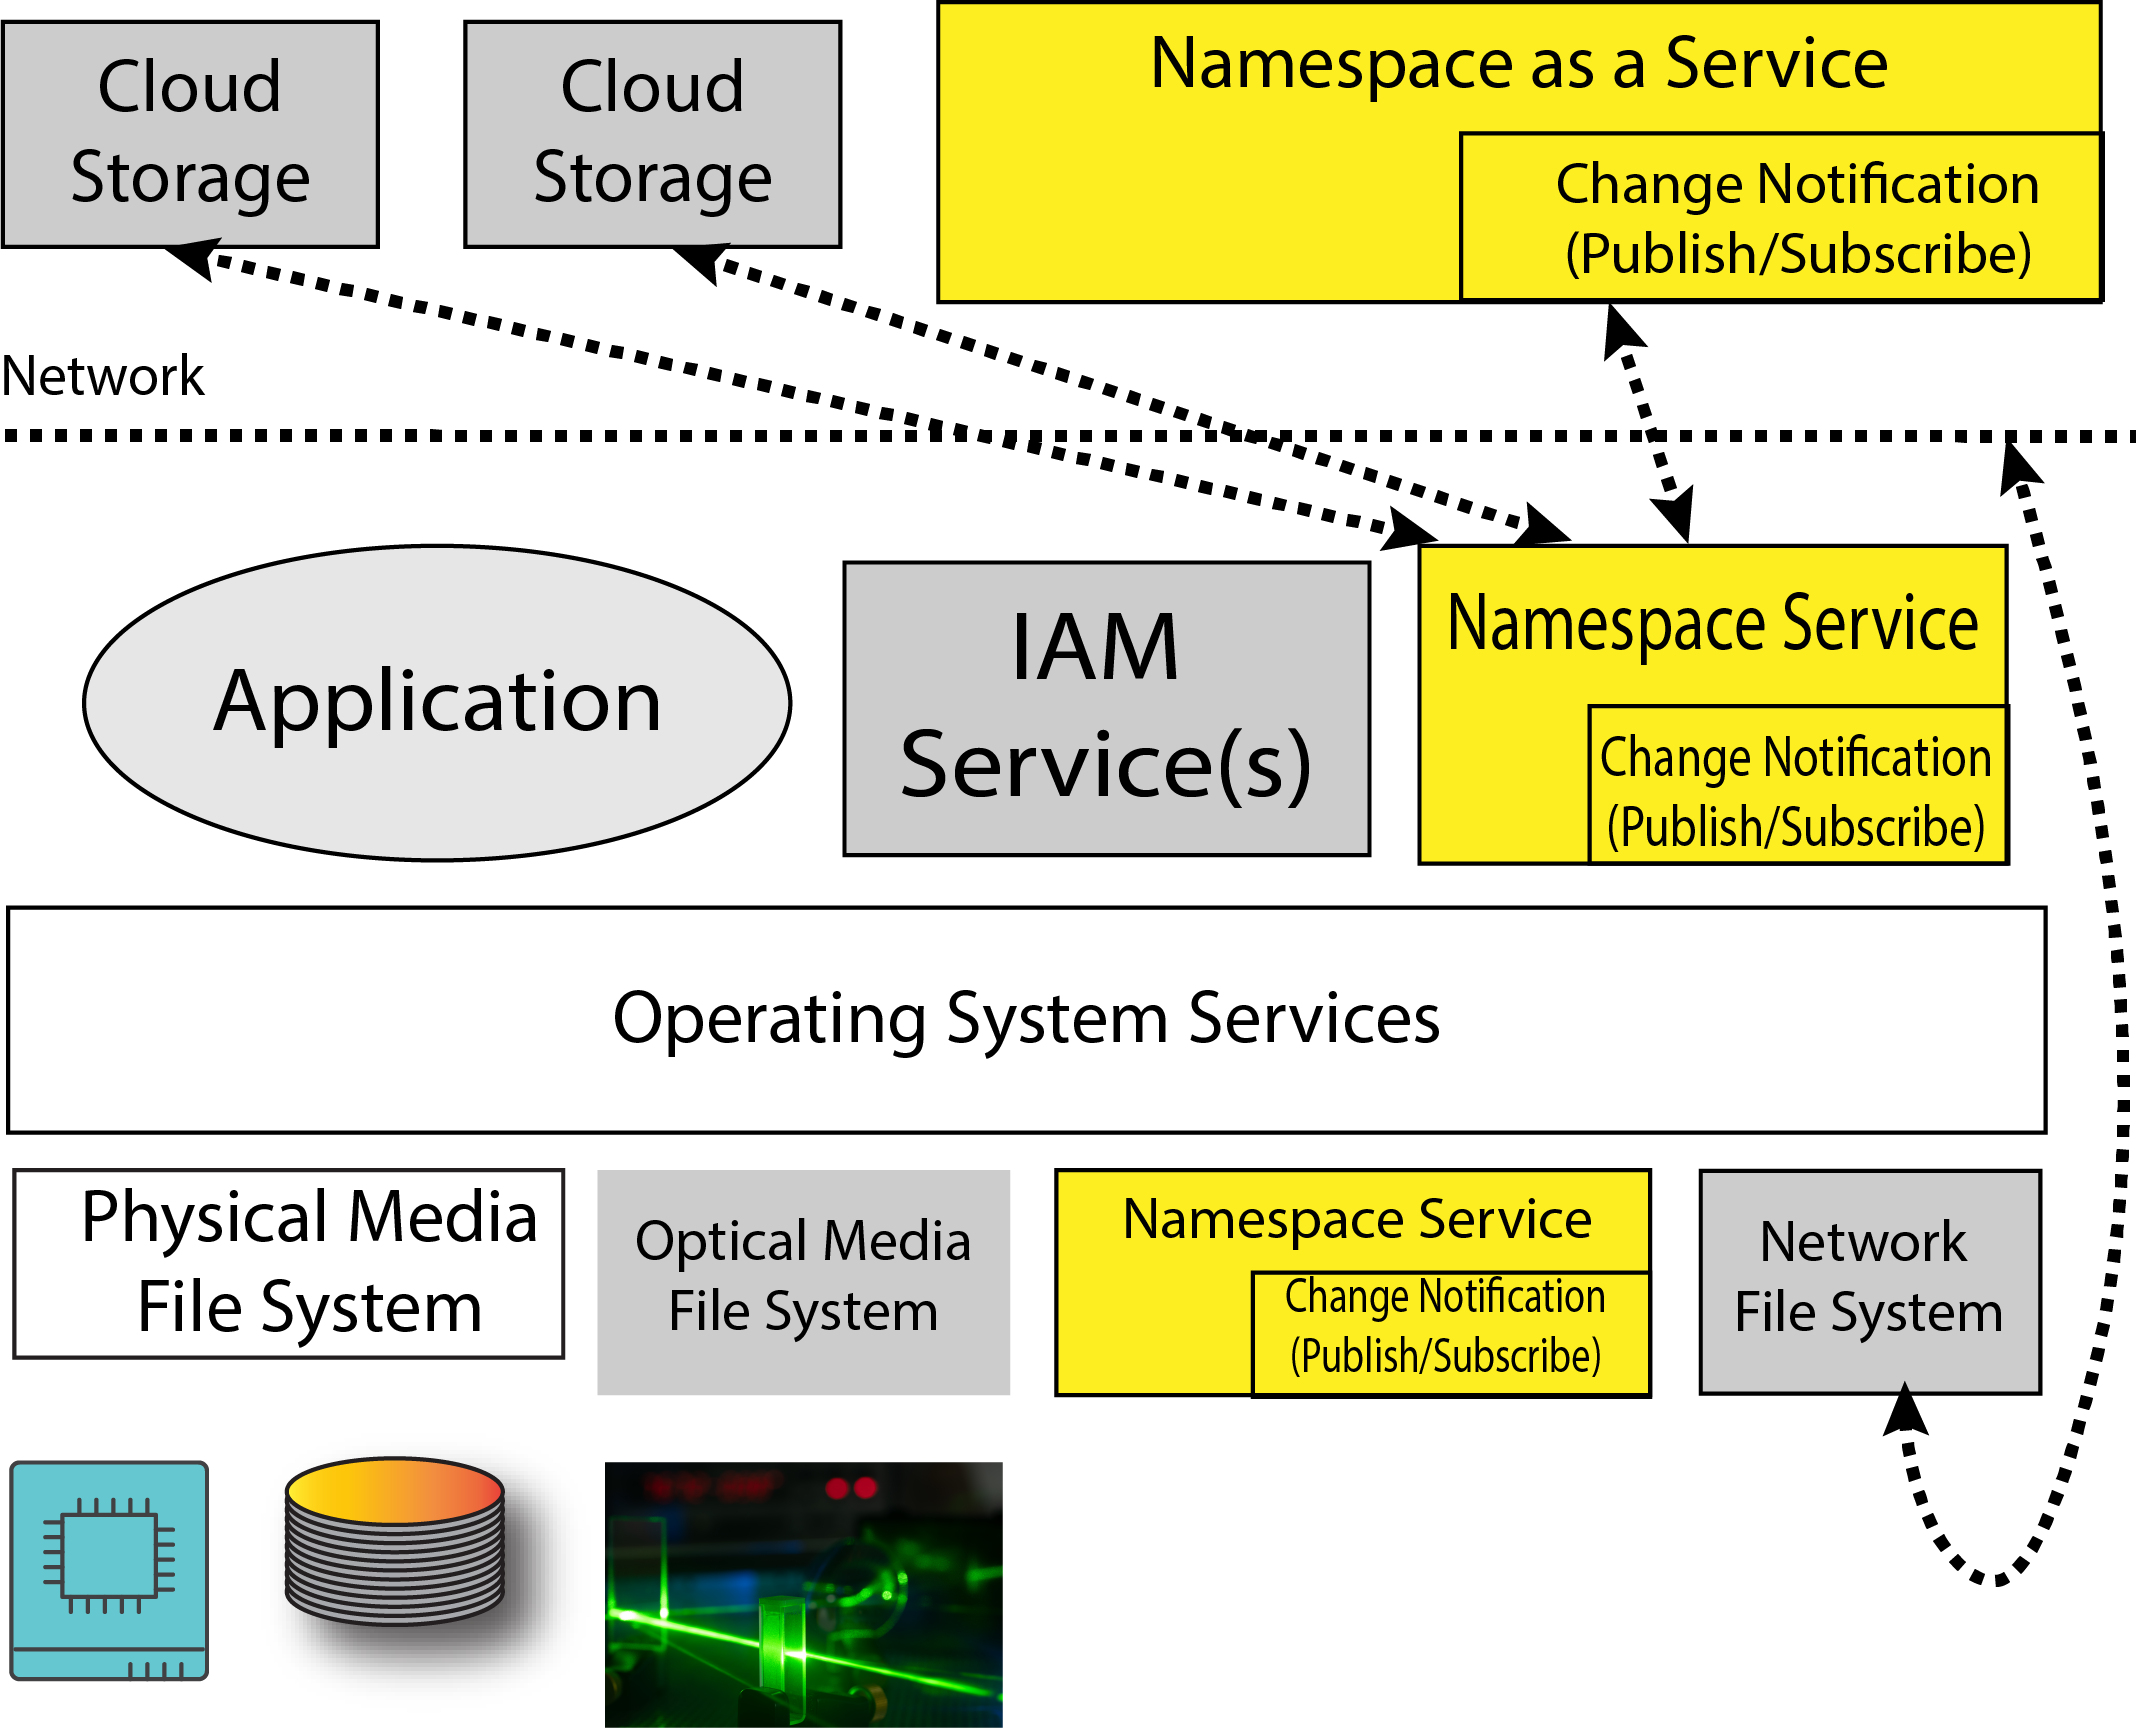
\includegraphics[width=0.95\columnwidth]{reference/hotos21/figures/nirvana-arch-8.png}
    \end{tabular}
    \caption{Nirvana Systems Architecture.}  %Separate Namespace service(s) from storage service(s).  Kernel namespace service permits use throughout OS lifetime, including boot.  User namespace service permits integration with remote namespace service and local namespace service, providing integration over the network.  Namespace as a Service (Naas) provides the ability to maintain shared namespaces across computational device boundaries; can provide primary or secondary name services.}
    \label{fig:systemsarchitecture}
\end{figure}

\subsection{Architecture}
\label{hotos21:architecture}

\newcommand{\REF}{reference}
\newcommand{\PROJECTION}{view}

\section{The Nirvana Architecture}\label{sec:arch}

%\begin{figure}
%  \begin{center}
%  \begin{footnotesize}
%    \begin{tabular}{|cp{0.75\columnwidth}|}\hline
%        silo & stores objects\\
%        object & the file's content\\
%        meta-data & the files attributes/properties\\
%        key & the unique identifier of the object\\
%        namespace & defines name context, high-dimensional attribute space \\
%        projection & construction a lower-dimensional namespace from a higher-dimensional namespace\\
%        name & a friendly/meaningful object name within the namespace. \\
%        locate & the process of obtaining an object's key within a context/namespace. \\
%        search & the process of locating an object based on a search query. \\
%        navigate & the process of locating an object based on following meaningful names \\
%        Overall & I think this is powerful: the user can define the namespace and its projections.
%    \\\hline\end{tabular}
%\end{footnotesize}
%    \end{center}
%  \vspace{-4mm}
%    \caption{Terminology (will go away for final submission)}
%  \label{fig:terminology}
%\end{figure}


% Surbhi asks that I include multiple cloud storage silos in the picture.  I wonder if we could add network file systems as well; I just didn't want them to be below
% the namespace.
% Puneet indicates that the text is too small.  We both agreed this needs to be centered and a bit larger (it feels like I'm wasting space).

%\mis{I did a commit before changing this section, but I wanted to tweak some terminology and provide a gentler introduction to this section. I worry that asking the reader to adopt a whole new terminology before telling them what we are really proposing is too great a burden.}
%\tm{I actually agree; defining the terms up front is, however, a useful tool for us when writing the text.}

We propose separating context/semantic naming from location and exposing this to users.
This separation will enable users to navigate/search data across multiple silos independent of where data is stored, and their organization preferences.
To realize this, we present the Nirvana architecture.
In Nirvana, storage silos need not change how they store objects, assign them silo-local \textit{location} names,
support their choice of attributes, and provide ways for users and other services to access them.
More interestingly, we absolve storage silos from providing \textit{context/semantic} names.
Instead, we introduce \emph{Nirvana namespaces} and \emph{namespace services}, which integrate one or more silos to provide \textit{context/semantic} names and access capabilities. In the following discussion, we use the term \emph{object} to refer to a discrete unit of storage, such as a file stored in an existing storage silo. Objects can reside on device-local file systems or in the cloud. Users access objects via requests to namespace services, which can be either local or cloud-based (see Fig.~\ref{fig:systemsarchitecture}).

\paragraph{Namespaces} In a Nirvana namespace, the name of a data object simply becomes a \textit{collection of metadata attributes}. Attributes are tuples consisting of, e.g., type, name, value, and author.
To date, we have identified three attribute types: \emph{authoritative}, \emph{annotated}, and \emph{autogenerated}.
Authoritative attributes are statements of fact provided by the silo, e.g., file size, creation time, content hash.
The author of an authoritative attribute is the silo containing the object; if the object is replicated in multiple silos, the author is the originator of the object.
Annotated attributes are provided by users or applications, e.g., Word document attributes, user-supplied tags, image metadata.
The author of such attributes is the user or program providing the annotations.
Finally, autogenerated attributes are produced by services, e.g., the cat video detector, a keyword extraction service.
Authors are responsible for defining the semantic meaning of their attributes.
Nirvana allows an unbounded number of attributes per object and requires only one: the authoritative location attribute,
which is a set of identifiers that refer to the silo and silo-local name(s) by which an object can be accessed.


%In the following discussion, we use the term \emph{object} to refer to a data element stored on and managed by Nirvana.
%Objects can reside on device-local file
%systems, network attached file systems (e.g., CIFS/SMB, NFS),
%distributed storage that projects onto a local storage silo (e.g., %OneDrive, Dropbox), and
%cloud storage systems of any type
%(e.g., Amazon S3, Azure Cosmos, Oracle Server, MongoDB).
%Users access objects via requests to namespace services, which can be either local or cloud-based services.\footnote{If a cloud-based services is used, we assume a caching layer on the local device to ensure access to data during disconnection. In the simplest case, the caching layer degenerates to the local file system namespace.}

\paragraph{Namespace Services}

The namespace service provides support for three basic operations: (1) the ability to create a Nirvana \REF, which is a set of metadata attributes;
(2) the ability to map a {\REF} to the underlying storage location and vice versa; and
(3) the ability to query the namespace to find {\REF}s that match a  pattern.  These {\REF}s are immutable: deletion is achieved using a tombstone and update by creating a new {\REF}, with a new creating timestamp.  This preserves history and allows versioning, assuming storage silo support.

% Moved from Intro to here.  See if we can capture it.
% Location is usually a one-to-one, or one-to-many relationship.
% Context/meaning are many-to-many relationships.

%A Nirvana namespace service runs on a local system or in the cloud, may work with an OS-integrated
A \textit{namespace provider} may also provide an API used by applications to interact with namespaces, allowing construction of new visualization and search tools.
For example, if you are searching from your smartphone, you can find a specific document, regardless of where
it is stored, whether that is your cloud storage system, a desktop computer, or some other storage location and even if it is not presently accessible.
Conversely, this model can be constructed to permit maintaining multiple distinct namespaces, so that each user is able to see \emph{{\PROJECTION}s} of their own data.

\paragraph{Locating specific objects} From our description so far, it seems that Nirvana is all about providing fertile ground for effective search, but it may be unclear how the user could \textit{locate} the specific object they need. We provide an example to illustrate how Nirvana can support this.

% Traditionally. Name and hierarchy of directories.
% In Nirvana, these can become attributes, and a namespace provider can simulate a legacy hierarchical namespace. Support users who find it useful and legacy tools, such as compilers.
% At the same time, allows users to gently depart from this model. For example, HPC community embed metadata elements of their objects into file names, users can now store these  elements explicitly with the name service, while also retaining the desired part of an old-fashioned name as a separate metadata element.

In traditional systems, a user gives a file a memorable name, e.g., \texttt{eddie.txt}.
In addition, hierarchical directory structure provides additional context for the object, helping the user locate the precise instance of \texttt{eddie.txt} that they need.
For example, there can be a \texttt{faculty/recommendations/eddie.txt} and \texttt{papers/fantasstic/eddie.txt}.
Nirvana supports locating objects via memorable names by assigning the object a user-provided attribute, e.g., \texttt{eddie.txt}.
Similarly, to simulate navigation by directory hierarchy, an object can be assigned attributes corresponding to the path components.
In this way, Nirvana can also support legacy tools relying on hierarchical directory namespaces.

At the same time, Nirvana can help users go beyond using memorable names.
For example, in the experimental science community, users traditionally embed the experiment context into the name of their data files~\cite{guo2012burrito}.
In Nirvana, users can explicitly store those metadata elements in a namespace.
Then, grepping for, say, \texttt{experiment-data.txt} can return multiple instances, but their metadata attributes can be explained via \texttt{stat}, and a \texttt{``diffstat''} command could also show the differences in the attributes between the two {\REF}s.

While hierarchical file system provide us with path and file names for search, our approach can make use of other augmented metadata elements, allowing us to narrow the results.

% (1) We don't lock ourselves into a set of attributes, so we don't need prescience. We don't need a big centralized indexer that knows all about all types of files.
% (2) We can customize these "tags" based upon the user's own behavior, and can be added to an indexing list.
% We can use the attributes to provide the "most relevant" results in the visualization tool(s).


\paragraph{Sharing, Access Control and Privacy}
% - access control  -> who can access the file, what part of the file, what attributes (all, just a subset, ?)
Enabling safe sharing requires a clear model of access control and a clear understanding of possible privacy implications.
While traditional file systems do have a vague notion of namespace access control using directory permissions, we are now faced with two explicit levels requiring access control: the object itself and the metadata.

What rights exist on each level and how do they relate to each other?
In Nirvana, possession of the {\REF} does not imply any rights to access the object, since access is managed by the storage silo itself.
The namespace provider has the ability to encode encrypted values within metadata elements, which also allows storing of sensitive information within the name without compromising security --- anyone with the Nirvana {REF} must still also have the relevant key to understand the value of specific attributes.
Similarly, this permits storing metadata in a third party service without compromising the contents of the metadata attribute.
%Utilizing digital signatures to protect the metadata element can be used to verify that the decryption key used is correct, or it can be used to verify that the value itself did originate with the specified authority to prevent spoofing.  This ability to secure individual metadata elements against tampering protects from malicious actors tampering with metadata elements as well as permits users to define their own unique rings of trust based  upon their own (or their organization's) criteria.

%Intuitively, a user may only perform an operation above if they posses the corresponding rights. There are two access control methods: access control lists and capabilities. Which form will prevail for namespaces and for the objects themselves?

%In addition, there might be certain rights a user needs to have in order to further share the object (or namespace) with other users or add the object to another name space. How can we revoke the rights from users and who is allowed to revoke -- is this an explicit right or implicitly given to the owner?

%Namespaces may contain many properties of their objects that in turn contain many bytes of data. Can we assign rights to particular properties or bytes?
%\reto{github access token}
%\tm{Remember in Twizzler, where they constructed objects via composition?  I'd argue that you \textit{could} do exactly the same thing and use it to control logical regions.  That's definitely not something we do with the existing APIs, but it could be something a file system permitted via a more flexible interface.}

%Given that a name in Nirvana includes the metadata necessary to locate the object in the global storage space using a URI, it is easy for names to be shared between namespaces.  There is no inherent requirement that the recipient of names need trust the metadata elements of that namespace in the same way the original owner did --- each user can define their own unique "rings of trust" with respect to individual metadata elements.

An important element of the Nirvana namespace model is the ability to identify not only the \textit{type} of a metadata attribute,
but also the \textit{authority} that provided such data.
To accomplish this, we need to have a mechanism for allowing verifiable identification for the metadata attributes that make up the name.
However, rather than propose a new identity and access management (IAM) service,
we simply note that we expect Nirvana to work with a least one such service (Fig.~\ref{fig:systemsarchitecture}).
In addition, this model also allows for a specific treatment of trust relationships that need not rely upon the namespace itself.
In essence, this allows the user to define their own ``security rings of trust.''

Nirvana Namespaces detect storage changes via a publish/subscribe model, similar to prior work~\cite{birman1987exploiting,9229638}.

\subsection{Research Opportunities}\label{hotos21:research}

%The use of namespaces has changed, though the design and implementation has not evolved substantially.  Recent initiatives by commercial
%entities such as Google, Amazon, NetApp, and Qumulo to improve naming within storage silos indicates we have reached the breaking point.
%While allowing per-silo namespace solutions is one possible future, we view it as important from the \textit{user} perspective to avoid
%this type of single-vendor lock-in.  However, to achieve our Nirvana model will require research to satisfy a number of outstanding
%questions that our design has raised.

%We identify five open areas: what is left of a file system when the namespace is removed, what operations should we support on namespaces
%versus on silos, what does access control look like, what are the implications of privacy and security, how can storage silos utilize meta-data
%to smartly optimize storage.

\paragraph{File System Evolution}
% - what's left of the file system if we have the two kinds of naming

With a distinct namespace implementation, we need to consider questions on how to optimize their interaction.
For example, should we permit the namespace implementation to store its metadata within the storage silo?
How can the storage silo access metadata from the namespace?  How can we optimize storage silos when
they are not burdened with the different needs of namespace and storage management?  Can we provide
mechanisms to notify the namespace when changes occur within the storage silo?
These questions arise because we separate the traditional, hierarchical file system structure we have known for more than a half century.
%Is there a better implementation for extended attributes such that other ecosystem can use them? The current implementation problems are not unique to our ecosystem but general.
%How will the layout of the FS change when we associate more user specific, application specific contextual metadata with files?
%Can the algorithms to access these be improved? For eg: can we provide a hook for user space functions to run to create the contextual metadata when the file changes?
% By separating the two kinds of naming in namespaces breaks with the traditional, hierarchical file system structure as we know it for half a decade. The question arises of what is left from the traditional file system?
% This seems to translate into concept of a ``thin-waist'' for storage, an object store like construct where the objects are retrieved solely based on their key.

%\subsection{Supported Operations}
% - operations (interoperability between name spaces)
Traditionally, users see storage as a convolution of location and its context within the storage, i.e.~the path of the file defining its location and context.
Performing a file system operation was reflected on both the file system context and the backing store at the same time.
A clean separation of this two concepts into the storage (location name) and namespace (semantic/context name) raises fundamental questions on what kind of operations are supported by each of those two concepts, how  they relate to each other, and how closely coupled they are.

%\paragraph{Store Operations}
%Store operations are applied on the object itself. Users should be able to create/delete objects, as well as read/write them.
%While those operations seem obvious, it is less clear for other aspects like rename and versioning: how does creating a new version or renaming it play together with the namespaces this object may appear in, and how do we refer to a particular version?
%Given users will use the namespace to search for their objects, does renaming even make sense?
%Based on the four operations mentioned previously, one can build more complex operations like copy or move to, for example, move an object to another silo.
%By doing so, should the object identifier be preserved? What happens if we forget the identifier?
%If not, how are we keeping the namespaces in sync with the new location of the object? Is there an equivalent for the HTTP 3xx status codes indicating temporary or permanent redirects?
%Lastly, users want to share access to objects, e.g.~for collaborative editing.
%We will talk about the rights and permissions involved in the next section with respect to sharing objects.

%\paragraph{Namespace Operations}
%Namespace operations are applied on the namespace. Similar to the objects, a user may want to create its own namespace, or delete it again if its no longer used. The central question here is where do these namespaces reside and how do we refer to a particular namespace?
%Is there some kind of namespace service, or are they running on a users local machine and thus may not always be accessible? Is there some kind of root namespace to find other namespaces? Is there some kind of register operation?

%Note, that an object may be added to to multiple namespaces, and it may be the case that the alst instace of it within an address space is deleted. What happens then? Can we even know that the last instance is deleted?

%Within a namespace, a user will likely want to add or remove objects, modify their meta-data information, and search the namespace for possible relevant objects based on a query or other objects with are alike a located one. What does it mean that two objects are relate?

%Besides searching, enumerating all objects that have been added to a namespace might also be desirable -- a potentially expensive operation. To what extent can we use the file contents to pre-populate the meta-data of the file? For example, CSCOPE builds an index of referenced symbols of source code files.

%Besides creating or deleting namespaces, a user may want to merge or unifiy two namespaces, or create a new subnamespace containing only the objects related to a project for instance -- an operation which may be expressed as create plus merge of a search result.

%Similar to the objects, a user may want to share an address space with other users to collaboratively work on a project, or because a business process requires approval of multiple people.

%Lastly, what is the interface to an namespace and how do they interoperate wich each other?


\paragraph{Differential Privacy and Security}
% - differential privacy & security (GDPR compliant)
The notion of access control mentioned above raises the question of how the security model used in this two layer system, as well as potential privacy issues: the meta-data may reveal much information about the object itself, even its presence, replication factor or temporary unavailability within a namespace is leaking information. How do we control this kind of information flow on the namespaces and the backing store?

Can we provide some form of differential privacy to the user of the name space? Effectively by prohibiting the user from enumerating the content of the namespace, and restricting queries to those who only produce one result -- in the sense you need to know precisely what you are looking for. As a more general aspect: how do we effectively prevent data leakage?

%In the context of privacy regulations like GDPR a user has the right to be forgotten. This implies we need to be able to not only find the relevant objects, but also the corresponding meta data. Is this feasible?
%Besides the namespace and object ownership, is there a concept of ``content'' ownership?
For example, in current namespaces there is no simple mechanism for finding all of the references to a specific object (e.g., the embarrassing photo that needs to be forgotten).
Nirvana provides the ability to find such references.  Can we create a GDPR compliance system that guarantees to expunge such references?


\paragraph{Using Metadata to Optimize Storage}
% - use meta data to organize the underlying storage
Currently, we have to explicitly decide on where we want to store our data by manually selecting from various data silos providing different properties, guarantees and methods of sharing.
Having a rich namespace containing meta-data for the objects, could we leverage this information to deduce the best method of storage?
For instance, the origin of the information may influence the selection of the data silo, whether data is to be encrypted, an expiration date assigned, creating multiple instances of the object in different silos, or whether we may want to keep track of different versions of the object.
Moreover, one may want to keep multiple, synchronized copies of the same object to support different access pattern or ensure locality.
How does regulation come into play (e.g., a object must not leave a certain jurisdiction)?
One of the central aspects of storage optimization is the question of which entity performs this?
This will likely require some form of synchronization among multiple namespaces that know about the object to ensure stability and avoid frequent changes to the storage.

\subsection{Conclusion}
\label{hotos21:conclusion}

We demonstrated providing useful ways to navigate/search across storage silos is not simply an HCI problem: it requires new system support.
We proposed Nirvana that, at its heart, separates location names from context/semantic names, and maintains those names in a cross-silo
name service separate but complementary from the storage. We presented research questions to address when building Nirvana.

% Nirvana

\section{HotStorage 2021}
\label{ch:appendix:section:hotstorage21}

\subsection{abstract}

Users store data in multiple storage silos, such as Google drive, Slack, email,
Dropbox, and local file systems that mostly rely on traditional user-assigned
names. A user who wants to locate a document that she saved while having a
conversation with her colleague on a specific subject last month will have a
hard time finding that document if she doesn’t remember in which silo it was
stored or what name it was given.

Prior work that introduced a \emph{Placeless} storage architecture enabled
cross-silo search using semantically meaningful attributes, while other prior
work used data provenance to construct a user's \emph{activity context} (e.g.,
what they were doing at the time they created or accessed data) to aid in
document location. We take a position that despite these prior systems that
demonstrated rich semantic search capabilities, we still cannot provide these
capabilities using existing system APIs and abstractions.

We explain that this is not simply an HCI problem and identify the systems
problems that must be solved to realize this vision. We present \emph{Kwishut}, an
architectural blueprint for enabling semantically rich, multi-silo data
management.

\subsection{Introduction}

Today's file systems provide two primary functions: a way to store chunks of data and names that provide users with the familiar
metaphor of a file cabinet (i.e., folders and documents).
Much has changed since we adopted this design.

Now most data resides not on local file systems but on myriad services such as
Dropbox, Google docs, Amazon S3, Microsoft OneDrive, and Github, as well as
attached to communication mechanisms and applications such as email, chat, and
collaborative communication platforms (e.g., Slack, Discord).

Today, just like local file systems, each of these storage solutions provides
its own storage and naming mechanisms. Pity the user Alice who wants to find the
file that was sent to her by Bob while they were having a slack conversation
about cool papers in HotStorage 2020, if she remembers neither the name of the
file nor whether she stored it in Dropbox, Google drive or her local file
system.

The \emph{Placeless} architecture~\cite{placeless-tois} provided an elegant
solution to this problem by enabling search across different storage silos using
semantically meaningful names. Each file was annotated with a rich set of
attributes, determined by the user or generated by software, and a naming
service, spanning silos, searched the entire collection of user files using
these semantically meaningful attributes. \emph{Placeless} was a huge
improvement over isolated storage silos and semantically-poor names, but it did
not solve Alice’s problem. Finding Alice's document requires that we track files
across storage silos and \emph{activity contexts}. An activity context describes
the other activities that were happening at the same time a document was
accessed. This context might include applications, such as Slack, email or a web
browser, which are not file systems in any traditional sense, but can be sources
and destinations for data and for its semantically meaningful context.

The only solution of which we are aware that captures activity context is
Burrito~\cite{guo2012burrito}, which used data provenance to keep track of a
user’s activity context, i.e., the applications they were running and actions
they were taking while examining a particular file. Unfortunately, Burrito is a
desktop application that was intended neither to work across multiple devices
nor to span multiple, remote storage silos. While it introduced the idea of
activity context sensitive search, it did not address any of the semantic
searching issues of Placeless and it did not consider the privacy consequences
of storing user context in a distributed environment.

We posit that \textbf{1) user naming should be entirely decoupled from local naming and 2) users need customizable and personal namespaces.}
We present \emph{Kwishut}\footnote{\emph{Kwishut} means ``naming'' in a native North American language.}, an architecture embodying this position, leveraging existing infrastructure where possible and extending it where necessary.
\emph{Kwishut} uses separate metadata and naming services coupled with user activity monitors.
\emph{Kwishut} is designed to allow incorporation of existing storage, metadata, and naming services without modification, while providing enhanced functionality when services support \emph{Kwishut} features.
We limit discussion to the systems infrastructure required to realize this vision; current storage management interfaces (e.g., file browser) can use \emph{Kwishut} namespaces directly, while the availability of rich metadata in \emph{Kwishut} enables HCI research on better ways for users to identify and find their data.

We begin with use cases motivating the need for \emph{Kwishut} (\S\ref{hotstorage:use-cases}), highlighting specific features missing from today's storage and naming services. Next, we present the \emph{Kwishut} architecture (\S\ref{hotstorage21:arch}) and future research directions it enables (\S\ref{hotstorage:future}).
We then discuss how \emph{Kwishut} builds upon prior work
(\S\ref{hotstorage:background}) and conclude summarizing our position (\S\ref{hotstorage:conclusion}).

\subsection{Why we need \emph{Kwishut}}
\label{hotstorage:use-cases}

%%%%%%%%%%%%%%%%%%%%%%%%%%%%%%%%%%%%%%%%%%%%%%%%%%%%%%%%%%%%%%%%%%%%%%%%%%%%%%%%%%%%%%%%%%%%%%%%%%%%%%%%%
\begin{table*}[!th]
    {\renewcommand{\arraystretch}{1.3} %<- modify value to suit your needs
        \begin{tabular}{p{0.11\textwidth}p{0.4\textwidth}p{0.425\textwidth}}
            \hline
            \textbf{Feature}                                                                                                                                        & \textbf{Existing Technologies} & \textbf{No Solution} \\
            \hline
            \usecaseactivitycontext                                                                                                                                 &
            timestamps and geo-location, image recognition, browsing history, ticketing systems, application-specific solutions like Burrito~\cite{guo2012burrito}. &
            Link related activity across apps, record  browsing history and chat conversations relevant to the creation of the data object, storing it in ways that are secure and compact.
            \\
            %
            \usecasecrosssilosearch                                                                                                                                 &
            Search by name, creator, content across silos,
            app-specific searches (e.g., Spotlight)                                                                                                                 &
            Unified search across all kinds of storage, including file systems, object stores, apps and devices
            \\
            %
            \usecasedatarelationship                                                                                                                                &
            De-duplication of documents, versioning of specific files, git ancestor relation                                                                        &
            Explicit notion of data identity, tracking different versions across different silos as data is transformed
            \\
            %
            \usecasenotifications                                                                                                                                   &
            File watchers (INotify), synchronization status, manually inspecting modified time                                                                      &
            Ability to subscribe to specific changes on attributes
            \\
            %
            \usecasepersnamespace                                                                                                                                   &
            Hierarchy plus hard/soft links. Use of tags.                                                                                                            &
            Creating personalized namespaces with with flexible data organization and views
            \\
            \hline
        \end{tabular}
    }
    \caption{Use-case driven functional requirements.}
    \label{hotstorage21:usecases}
\end{table*}
%%%%%%%%%%%%%%%%%%%%%%%%%%%%%%%%%%%%%%%%%%%%%%%%%%%%%%%%%%%%%%%%%%%%%%%%%%%%%%%%%%%%%%%%%%%%%%%%%%%%%%%%%

%Each storage silo provides a specific set of features facilitating certain use-case scenarios, for example, the local disk provides offline access to data, while cloud-based solutions allow users to collaboratively work on a shared document.

We identified five categories of information that are necessary to facilitate the integration of semantically meaningful naming with user activity context.
Unfortunately, to varying degrees, these features cannot be provided by today's storage system architecture.
We introduce these categories, summarize them in table~\autoref{hotstorage21:usecases},
and then present use cases demonstrating how they facilitate data management.

\subsubsection{Feature Wish List}
\label{hotstorage:features}
\noindent\textbf{Activity Context: }
As Burrito demonstrated~\cite{guo2012burrito}, the \emph{context} in which data were accessed or created is often a useful attribute on which users wish to search, e.g., ``\emph{I'm looking for the document I was editing while emailing \persa about their favorite wines}.''
To the best of our knowledge, there is no modern system that supports queries using rich context across applications.
We might be able to use timestamps or application-specific tags or history information in queries, but it is laborious, if not impossible, to intersect data from multiple applications and/or multiple silos.

\noindent\textbf{Cross-Silo Search: }
Users share documents in myriad ways: via messaging applications, on cloud storage services, and via online applications. Users should not need to remember which mechanism was used to share a particular document and should have some easy way of organizing and searching through a collection of such distributed documents.

\noindent\textbf{Data Relationships: }
Documents can be related in arbitrary ways. This relationship information can be used to facilitate and enable better search results. So far, we have identified three specific relationships that are particularly important:

\noindent\emph{1) copy} is a bit-for-bit identical replica of some data, in other words two items with different names store the same data.
% Deduplication functionality in storage systems frequently takes advantage of the prevalence of copies to reduce storage consumption. However, knowing that two items with different names are, in fact, the same is also valuable information for users.

\noindent \emph{2) conversion} is a reversible, repeatable transformation that changes the representation of data, without changing its semantics, e.g., converting a CSV file into JSON.

\noindent \emph{3) derivation} refers to data that has been computationally derived from another object by altering its content, e.g., adding a row to a spreadsheet.

While storage systems can recognize copies, they cannot distinguish conversions from derivations. However, from a user's perspective, these operations are quite different: a conversion can be repeated, which is not necessarily true of a derivation.

\noindent\textbf{Notifications:}
Users frequently want to be notified when documents change, and many storage services offer this functionality.
However, users might also want notification when data on which they directly or indirectly depend changes. This requires both a notification system and an awareness of the data relationship between different objects.

\noindent\textbf{Personalized Namespaces:}
Users have different preferences and mental models to organize their documents, a source of conflict in a multi-user setting. We need a way to provide each user the ability to personalize their document structure.

\subsection{Use Cases}
The following use cases illustrate how the features described above arise in common place activities.

\noindent\textbf{Data Processing:~}
\persa and \persc are preparing a report summarizing their work on a data analysis project for a customer.
\persc sends an email to \persa containing a CSV file with original data.
\persa opens this document in Excel, formats and filters it, adds additional data from a corporate storage silo,
and then returns the Excel document to \persc on Slack.
\persc is away from their desk when it arrives, so they open it on their phone, uploading it to a cloud drive.
\persc then sends the link to \persa for editing with update notifications.
Finally, \persc sends a PDF of the report to the compliance officer who promptly asks, ``Where did this data come from?''

\noindent\textit{Feature Analysis:~}
This use case highlights the need for 1) \usecasedatarelationship, as it has instances of copies, conversions and derivations, 2) \usecasecrosssilosearch, as these items are located in multiple silos and accessed by multiple devices, and 3) \usecasenotifications, as update notifications need to be distributed to designated users.

\noindent\textbf{Delete Request:~}
Some time later, the compliance officer requests that all documents containing a customer's data must be deleted.
To help with finding all relevant customer data, \persb joins the project and examines the report and requests the original data from which it was produced.
\persa remembers that they gave the original data to \persc shortly after collecting it, but does not remember the name, location, or even how the relevant files were transmitted. Thus, \persa has to manually search possible locations and applications, sendsing references to documents to \persb, who then starts organizing these files to methodically identify the ones that might contain the customer's data. In the process, many of the other team members' references to the documents stop working.

\noindent\textit{Analysis:~}
This use case illustrates the need for 1) \usecaseactivitycontext to capture
data that has been collected while interacting with the customer, 2)
\usecasedatarelationship to identify related documents, 3)
\usecasecrosssilosearch to easily locate relevant documents across data silos,
and 4) \usecasepersnamespace to create a individual data organization.

% \noindent\textbf{Security and Privacy:~}
% \persg, an investigative journalist who routinely receives sensitive information from third parties, is investigating the company from the prior use cases.
% \persg needs to be able store and access sensitive information, including information about the activity context of various e-mails, documents, pictures, and audio and video files.
% While \persg ensures that these data are encrypted, they need to also ensure that they can both find information and ensure that meta-data associated with those files is both usable and properly protected across silos.

% \noindent\textit{Feature Analysis:~}
% This case requires both \usecasecrosssilosearch and
% \usecaseactivitycontext to allow \persg to gather information obtained from specific meetings or at a given time/place.
% While \persg must protect their sources, they must also be able to associate evidence with those sources to make judgement calls about their validity, so we must design security and privacy policies for attributes that accomplish both.

\subsubsection{From Use Cases to Architecture}

Each use case and feature class suggests capabilities that are unavailable
today.

In~\autoref{hotstorage21:usecases} we identify existing technology that can be brought to
bear on the problem while teasing apart the precise details that are missing.

Repeatedly, we find that critical information necessary to provide a feature is
unavailable, that providing such information is non-trivial, and that obtaining
it creates a collection of privacy challenges.

\subsection{Architecture}
\label{hotstorage21:arch}

\begin{figure}[!tb]
    \centering
    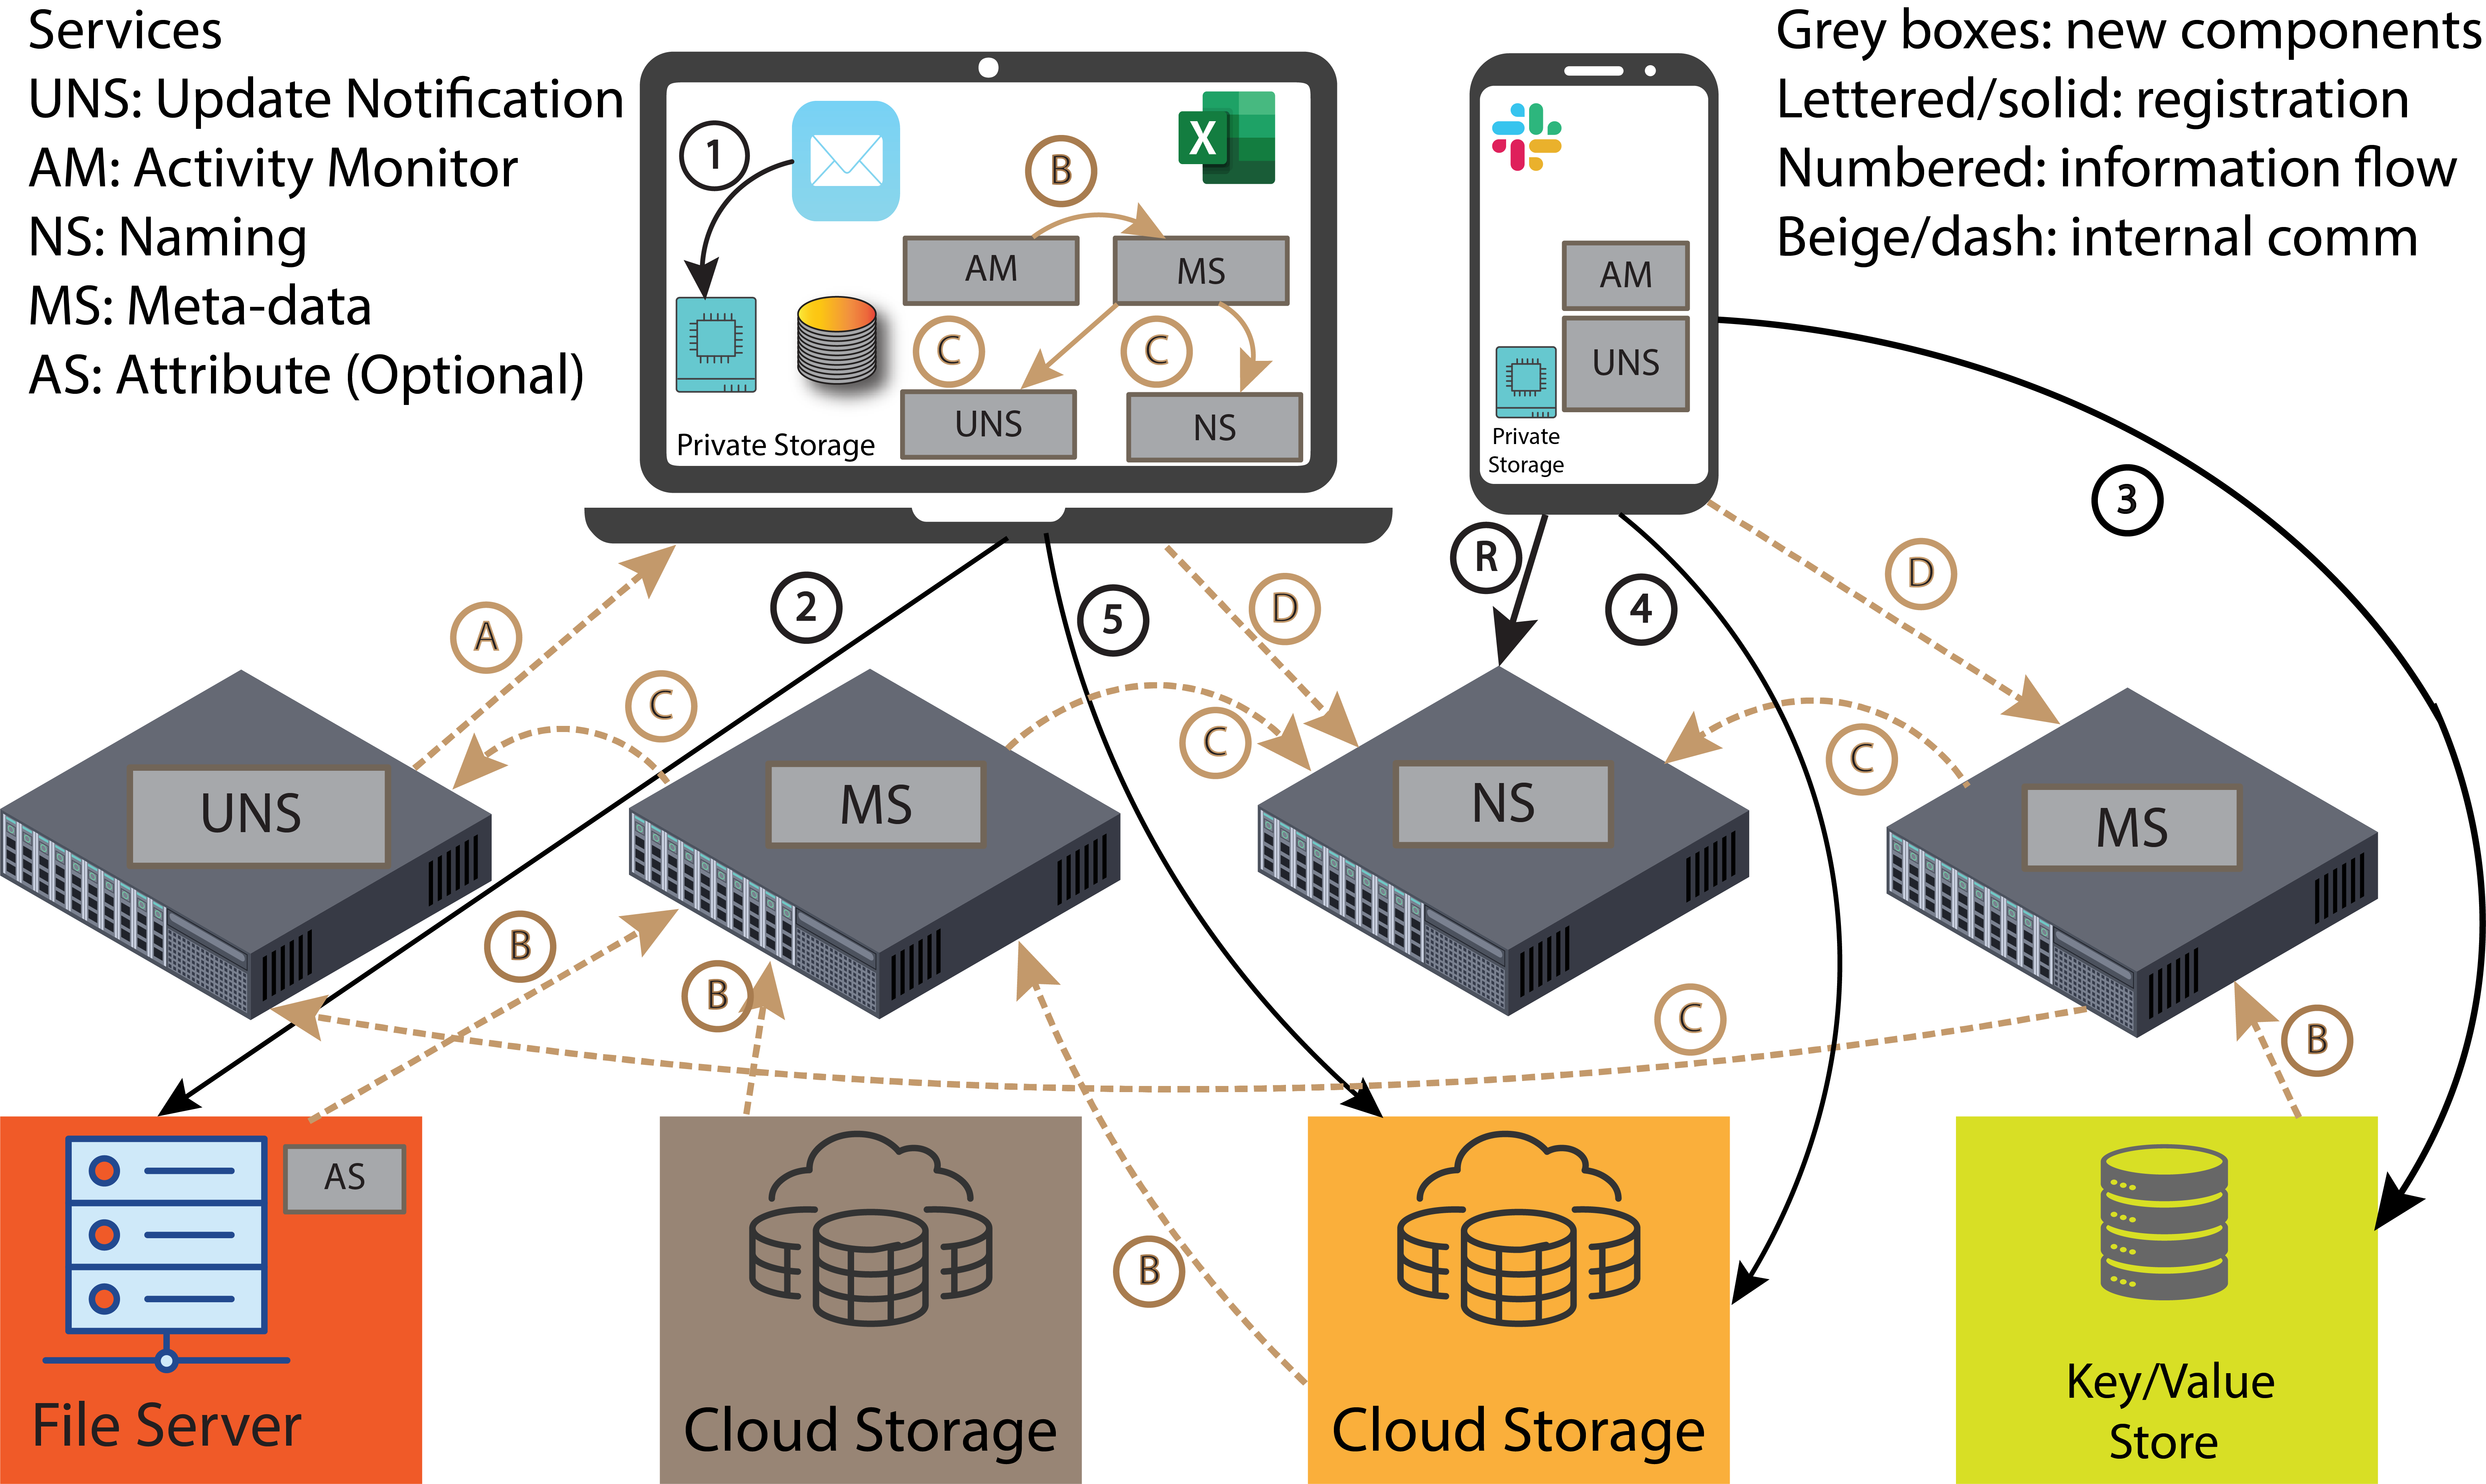
\includegraphics[width=0.45\textwidth]{reference/hotstorage21/figures/Naming5-legend.png}
    \caption{\emph{Kwishut} Architecture (\S \ref{hotstorage21:arch}).
        %Grey boxes indicate new components. AM=``Activity Monitor'', MS=``Meta-data Server'', UNS=``Update Notification Server'', NS=``Namespace Server''.
    }
    \label{fig:arch}
\end{figure}

%\reto{Using meta-data service that must inter-operate (federated meta data) and relationships are not first-class citizen, cannot glue the meta-data service together with naming services to enable the things we want to do. }
%\reto{the storage location is independent on the notion of related files: meta-data service treats relationships as first-class citizens. }
%\reto{get the attributes out of the silos --> currently: this is done manually}

\emph{Kwishut} is a family of services that enable sophisticated search and naming capabilities.
The key features that differentiate \emph{Kwishut} from prior work are:
\textit{1)} incorporating object relationships as first class meta-data,
\textit{2)} federating meta-data services,
\textit{3)} recording activity context,
\textit{4)} integrating storage from multiple silos, and
\textit{5)} enabling customizable naming services.
Data continues to reside in existing and to-be-developed storage silos.
\emph{Kwishut} interacts with these silos, collects and captures metadata, and
provides a federated network of metadata and naming services to
meet the needs of the use cases in \S \ref{hotstorage:use-cases}.

\subsection{\emph{Kwishut} Services}

Figure \ref{fig:arch} illustrates the \emph{Kwishut} architecture. \emph{Kwishut} allows for
different deployment scenarios. The five services can be run independently, they
can be co-located and bundled together to run on a local device, integrated into
an OS, or available as web-based services.

In the discussion below, parenthesized numbers and letters refer to the arrows
in Figure \ref{fig:arch}. There are five main components:

\noindent\textbf{1) Metadata servers (MS)}
are responsible for storing attributes and provide a superset of capabilities found in existing metadata services~\cite{federatedMetaData,smartstore}. Users can register an MS with activity monitors or attribute services, which allows the MS to receive updated attributes from storage objects and activities (B). Thus, there can be multiple sources of attributes including the user itself. Metadata servers may retain the full or partial history of attribute updates or maintain only the most recent value.

\noindent\textbf{2) Namespace servers (NS)}
connect to one or more MS and use the metadata to provide users with a
personalized namespace that allows both manual organization (i.e., a
hierarchical namespace) and rich search capabilities.
Users can register with an NS (R) that uses one or more MS to obtain relevant
attributes from them (C). Additionally, users can be part of a corporate NS that
allows sharing of their select metadata with other users via standard enterprise
public-key cryptography.


\noindent\textbf{3) Activity monitors (AM)}
run on the user's devices. Their main function is to observe temporal relations,
activity context, and relationships between objects on a user's device and
transmit them to an MS (D).


\noindent\textbf{4) Attribute services (AS)}
extract attributes from storage objects and transmit them to an MS (B). An AS
might be invoked on updates, run once or periodically. For example, a file
system AS would update the object's metadata with basic attributes such as size
or modification time. There can be many AS that extract more ``interesting''
attributes, e.g., image recognition, similarity, or other classifiers.

\noindent\textbf{5) Update notification server (UNS)}
provides notification mechanisms. Users can register interest in changes of
attributes or underlying storage and will receive a message on change events (A)
to which they have access.

\subsection{\emph{Kwishut} working example}

To make the \emph{Kwishut} architecture concrete, we revisit our use-cases from
\S\ref{hotstorage:use-cases} and walk through parts of it to illustrate how \emph{Kwishut}
supports the various actions and events.

\noindent\textbf{Storing the e-mail attachment.}
\persa's act of saving the CSV file that \persc sent in email corresponds to the creation of a new object on the file server silo, i.e., the file system (4). The file server is \emph{Kwishut}-aware, so the AS co-located with it extracts attributes from the document and forwards them to the MS (B).

The AM on \persa's laptop detects that the CSV file came via company email from
\persc. It then captures the activity context identifying the relationship
between the e-mail and the CSV file and transmits it as additional metadata
about the CSV file to the MS (that already contains metadata extracted by the
AS). Moreover, because there is a company-wide namespace service, \emph{Kwishut}
establishes that the e-mail attachment, the CSV in the file server, and the one
on \persc's laptop (from which the file was sent) are exact copies of each
other.

Many applications already record some form of activity context, e.g., chat
history, browsing history. Such histories provide a rich source of additional
metadata. Other activity context, specifically the relationship between objects,
such as the fact that a particular file was saved to a local storage device from
an email message, requires more pervasive monitoring as found in, e.g., whole
provenance capture systems~\cite{camflow}. \emph{Kwishut} is agnostic about the precise
data that comprises activity context, but allows for storing and accessing
activity context as metadata.

\noindent\textbf{Creating the Excel file.}
Next, \persa opens the CSV file using Excel and stores it as a spread sheet.
This creates a new object. The AM detects that the newly created spreadsheet is
a conversion from the CSV file, either via a notification from \emph{Kwishut}-aware
Excel or by monitoring the system calls executed on the local system. \persa
proceeds to modify the data by filtering it in Excel and saving the changes. The
AM records this event and updates the meta-data of the spreadsheet to record the
derivation-relationship. Ideally a \emph{Kwishut}-aware version of Excel specifies to
the AM the exact type of the relationship (in this case a derivation); otherwise
the AM informs the MS about an unspecified data relationship by observing the
opening of a CSV file and a subsequent creation of the Excel file.

% \persa proceeds to upload the new Excel file on Slack, which triggers the creation of a new storage object as Slack creates a local copy, the addition of new metadata to MS via AS, and the addition of a \emph{copy} data relationship between the original Excel file and the Slack’s copy. The AM notices (by monitoring Slack chat) that the file was shared with user \persc and promptly notifies the MS, which adds this detail to its metadata.
% Once \persa is done, its local MS has been updated with three new objects: the CSV file, the corresponding Excel file, and Slack’s copy of the Excel file. There is a data relationship linking all three, and the metadata informing us that the original CSV came from \persc and that the final Excel file was also shared with that same person. If \persa wanted to remember what happened to the the data from the original CSV from \persc, they could query their local personal NS, which would track down this history by querying the MS metadata.

\noindent\textbf{Sharing the spreadsheet.}
As \persc  receives the Excel file from \persa via Slack on their phone, a
sequence of metadata events similar to those described earlier takes place,
except the phone does not run a local NS or MS. \persc now uploads the file to
the company's cloud drive (4). The MS (by way of AS) reflects the creation of a
new object and records its remote location. The use of a company-wide namespace
and metadata service enables \emph{Kwishut} to record that the file in the cloud drive
is, in fact, a copy of the one received via Slack.  Further, \persc informs
their personal NS that they wish to notify \persa about all updates to the file
on the cloud drive. Thus, whenever an AS sends updated attributes to the MS,
\persc receives a notification.

% The sharing relationship between the personal NS of \persa and \persc, and the exchange of the relevant cryptographic credentials, would have been set up earlier.

\noindent\textbf{Data origin and delete requests.}
When the compliance officer asks about the origin of the data, \persc can query
the corporate NS to obtain the complete history of the report. This includes the
spreadsheet from which the report was derived and the e-mail or Slack messages
that transmitted the files.
The corporate NS was configured to be aware of the locations of the
collaborating users' personal NS. Moreover, because of the activity contexts
captured by the AM, \emph{Kwishut} is able to identify documents that were created
during any activity involving the customer whose data must be deleted. Starting
from these documents, and by using the relationship of documents, \persb was
able to find all relevant objects and delete them, including the e-mail and
Slack messages.


% \persa would have configured their personal NS to allow sharing of the metadata associated with \persc with their corporate NS, and \persc would configure their personal NS similarly. As a result, when \persc issues to the corporate NS a query asking to trace the origins of the data in the final report, the corporate NS is able to return all the history tracing back to the original CSV file.

Note that unlike existing systems, \emph{Kwishut} is able to efficiently find related
objects across storage silos. Operating systems already provide users with
indexing services to accelerate search of local files. This search can be made
cross-silo by mounting and enabling indexing on network shares (e.g., Windows
Desktop Search), or by interfacing with specific applications such as e-mail
(e.g., MacOS Spotlight, or Android search). The problems with indexing on a
large network storage repository are resource limitations such as bandwidth and
local storage that may render the system unusable during indexing. In contrast,
\emph{Kwishut} addresses these limitations by delegating indexing and storage to one or
more services.

NS are responsible for providing efficient search functionality. \emph{Kwishut} uses AS
to keep attributes up to date with object modifications. Lastly, \emph{Kwishut}
supports coordinated search among one or more local and remote NS, allowing, for
example, a user to search across both their local NS as well as their employer's
NS.


% \sasha{There are a few remaining pieces that we did not mention. Please look at the commented text at the end of architecture-new.latex to see if you want to restore some of that text.}
%\subsection{The remaining pieces}

%To complete the description of \emph{Kwishut} here we fill in some of the missing details.

%\textbf{Metadata deletion and updates.} Metadata associated with a storage object can be deleted underlying storage object is deleted or when the user is required to comply with legal requirements, such as the “right to be forgotten”. The metadata of the object is updated (via push or pull by the AS) if the object changes in the underlying storage silo or if the user (or \emph{Kwishut}-aware applications) choose to create additional metadata, e.g., run image recognition on photo files and record the names of identified places and persons.

%\textbf{Security} \sasha{I am just copying what we had in the original document, but I don't know if this is useful. Cut this? } We base our security requirements on a simple threat model that considers (1) protection of the meta-data itself and (2) protecting information that might be gleaned from activity within \emph{Kwishut}.  We assume the primary threat here is inadvertent disclosure, particularly through the use of third-party service providers. Secondary threats include the ability to verify attribute information provided by external parties, including anti-repudiation as well as tampering. \MIS{I don't understand that last sentence; do you meant that the threat is attribute spam?}

%Using public key mechanisms for signing attributes provides a standard mechanism for verifying the authenticity of the attribute itself; forged signatures can be detected using other information from the \emph{Kwishut} object.  For example, an object stored in a given silo would require use of a known set of digital signatures from the relevant authoritative name service. \MIS{That last sentence seems backwards to me; I don't understand our claims.}

%\textbf{Data relationships} While \emph{Kwishut} treats the designated data relationships automatically, users and applications can create metadata for other relationships. For example, the corporate compliance officer might find it helpful if implementations of data security policies were explicitly linked to the appropriate regulation or mandate.

\subsection{Future Directions}
\label{hotstorage:future}
We now explore a few research directions that \emph{Kwishut} suggests.

\noindent\textbf{Attribute Security and Integrity.}
\emph{Kwishut} decouples naming and attributes from the storage object. This opens up a
research direction on the security model of attributes themselves. Are the
permissions on the attributes similar to the ones on the storage objects
themselves? Can a user change an attribute in its local namespace, but not in
the company wide one? This segues into the question of attribute
integrity/quality: not all attribute sources have the same trust-level. For
instance, a user might label an image ``dog,'' while the image recognition AS
might label it ``cat''.

\noindent\textbf{Privacy.}
\emph{Kwishut} collects a lot of metadata across multiple communicating channels and
storage silos, including activity data. This raises the question of how to
manage these metadata in a privacy-preserving manner.

\noindent\textbf{Interface Design.}
We presented a system architecture that provides a rich context to search and
organize storage objects. We envision that this will provide the foundation for
new directions in HCI research: By using individual namespaces, we can
dynamically organize and visualize documents and other storage objects, and
seamlessly navigate and locate related documents providing a new user
experience.

\noindent\textbf{Relationship-based Queries.}
\emph{Kwishut} tracks relationships between storage objects. These relationships
provide minimal data provenance~\cite{provprimer} allowin users to locate the
chain of related documents originating in a specific activity context.

These relationships are most naturally expressed as graphs, where nodes are
objects, and edges are the relationships between objects. Edges could have
weighted-labels, indicating the type and importance of their relationship.

This enables more sophisticated data-analysis beyond pure content-based indexing
by using graph queries.

For instance, lineage queries (i.e., tracing the history of an object) are path
traversals, which are challenging to implement efficiently in conventional
storage systems. This suggests that the NS and/or MS require sophisticated
storage and query mechanisms.

\subsection{Related Work}
\label{hotstorage:background}

\emph{Kwishut} draws on prior work in semantic file systems, using search to locate
documents, and federated naming systems.

\noindent\textbf{Semantic File Systems.}

Although we introduced our desire for semantically meaningful names with
reference to the Placeless architecture, the idea originated in the systems
community with the semantic file system~\cite{giffordSFS}, SFS.

SFS used automatically extracted attributes to construct virtual directories
that contained collections of semantically related documents.

There exist many extensions or variants on this theme such as per-process
namespaces~\cite{plan9}, inverting the database/file system layering to build
file systems on top of queriable databases~\cite{inversion},
manually tagged file systems~\cite{tagfs},
constructing semantic metadata stores from distributed
storage~\cite{smartstore}, and systems that manage conventional and semantic
structures in parallel~\cite{gfs}.
\emph{Kwishut} represents another step in this evolution.
It extends prior work by combining semantic naming with user activity context
and is designed for today's multi-silo'd storage encompassing everything from
mobile devices to desktops to object stores to cloud storage.


\noindent\textbf{Search.}
An alternative to creating a semantically meaningful name space is to enable extensive metadata-based search.
Desktop tools such as Apple’s Spotlight, Linux KDE Baloo, and Windows
Desktop Search adopt this approach.
However, breakthroughs in web search (i.e., incorporation of pagerank~\cite{page1999pagerank}) demonstrated that the relationship among objects is at least as important as the metadata itself.
The efficacy of provenance-assisted search~\cite{provsearch,uprove2,pindex} demonstrates that history, in addition to relationships enhance users' ability to locate documents.
However, searching for documents is fundamentally different from naming.
Search-based approaches rely either on a user to select the correct item from many presented or on the sufficiency of providing \emph{any} relevant document.
However, naming requires the ability to identify a specific document. \emph{Kwishut} is designed to support both searching and uniquely identifying a specific document.

\noindent\textbf{Multi-silo Data Aggregation.}
%\MIS{There is an entire market for consultants who help people manage data in multiple silos; who knew?}
%\MIS{It seems that the biologists are also really interested in multi-silo search.}
UNIX mount points~\cite{unix} are perhaps the first instance of federating namespaces.
Distributed federation, as provided by distributed file systems such as NFS~\cite{nfs} and AFS~\cite{howard1988scale} followed soon after adoption of local area networks.
With the advent of cloud storage, there has been work in federated namespaces that span
cloud stores~\cite{scfs,federatedMetaData}.
Nextcloud (\url{https://nextcloud.com}) allows users to connect multiple Nextcloud instances and integrate with
FTP, CIFS, NFS and Object stores. Yet, documents are still organized in a classic
hierarchical structure. Peer-to-peer sharing networks (e.g., IPFS \cite{benet2014ipfs}) implement a distributed
file system where nodes advertise their files to users.
MetaStorage~\cite{metastorage} implements a highly available, distributed hash table,
% similar to Amazon's DynamoDB, %% trying to cut a line or two to get us under the limit and if we leave this here, it needs a reference
but with
its data replicated and distributed across different cloud providers.
% MetaStore offers a key-value store interface.
Farsite~\cite{Adya:2003:Farsite} organizes multiple machines into virtual file servers, each of which acts as the root of a distributed file system. Comet describes a cloud oriented federated metadata service~\cite{federatedMetaData}.

\subsection{Conclusion}
\label{hotstorage:conclusion}

We have presented our position that we need \emph{Kwishut}, a storage
architecture that decouples naming from the storage location of documents and
data objects, provides customizable and personalized namespaces, and that makes
relationships between documents a first class citizen. With \emph{Kwishut},
users will be able to organize, share and find their data conveniently across
multiple storage silos using a rich set of attributes breaking away from the
rigid, hierarchical organization.

We expect \emph{Kwishut} will enable a broad area of research in HCI exploring
new ways to visualize and interact with data using the mechanism's provided by
\emph{Kwishut}. Moreover, we expect \emph{Kwishut} to provide interesting
scenarios for security and privacy research in storage systems.
